\section*{Introduction du chapitre}

    Dans la partie précédente, nous avons traité de la démarche scientifique appliquée pour la thèse, du point de vue épistémologique, éthique et méthodologique. Nous présentons maintenant les résultats obtenus sur le terrain. A partir de deux études, nous cherchons à caractériser les pratiques des \oess en matière de communication et d'action environnementale.  \\

    Ce chapitre est consacré à l'étude de la communication des entreprises sur le réseau social en ligne Twitter. L'intérêt d'étudier le discours, et en particulier un discours sur un réseau informel (par opposition à des documents comme des rapports annuels ou des revues de presse qui sont construits méthodiquement, relus et validés par plusieurs échelons de management), est de rendre compte de l'importance de l'environnement pour l'ESS et de la façon dont ce sujet est traité. L'action environnementale est-elle vue comme une contrainte, comme un atout et une opportunité ou comme une finalité ? En nous appuyant sur une méthode innovante, celle de l'exploration de texte, nous mettons en évidence les grandes thématiques environnementales abordées par les organisations, mais aussi les différentes stratégies rhétoriques retenues par les différentes structures de l'ESS. \\

    L’étude porte sur un échantillon constitué de 1 110 comptes d’utilisateurs répartis en 8 catégories. Le Tableau \ref{table:categoriesutilisateurs} détaille cette répartition. Les associations représentent près de la moitié des organisations de l’échantillon. Ceci s’explique par la très forte prépondérance de ce statut dans l’ESS où les associations représentent 93,9 \% des entreprises et 77,7 \% de l’emploi \parencite{observatoire_national_de_leconomie_sociale_et_solidaire_france2017atlas}. La relative sous-représentation des mutuelles dans l’échantillon s’explique par leur faible présence sur Twitter. La majorité des comptes de mutuelles correspondent à des fédérations (telles que la Mutualité Française).

    \begin{table}[h]
        \caption{Catégories d'utilisateurs}
        \label{table:categoriesutilisateurs}
        \centering
        \begin{tabular}{|l|r|}
        \hline
            \textbf{Catégorie} & \textbf{Nombre d'utilisateurs} \\ \hline
            Association & 544  \\ \hline
            Coopérative& 191  \\ \hline
            Fondation& 114  \\ \hline
            Fédération et Organisme de représentation & 111  \\ \hline
            Entreprise sociale& 73  \\ \hline
            Mutuelle& 50  \\ \hline
            Autre& 27  \\ \hline
            Total& 1 110  \\ \hline
        \end{tabular}
    \end{table}

    Au total, 910 649 tweets originaux sont collectés, sur une période allant du mois d’août 2008 à fin juin 2017. Comme le montre la figure \ref{figure:tweetsparannees}, le nombre de tweets augmente fortement d’année en année et la majorité des tweets se concentre sur la période récente (2012 à 2017). Les données sont réduites à 23 221 tweets identifiés comme traitant des questions environnementales.

    \begin{figure}
        \caption{Nombre de tweets collectés par année}
        \label{figure:tweetsparannees}
        \centering
        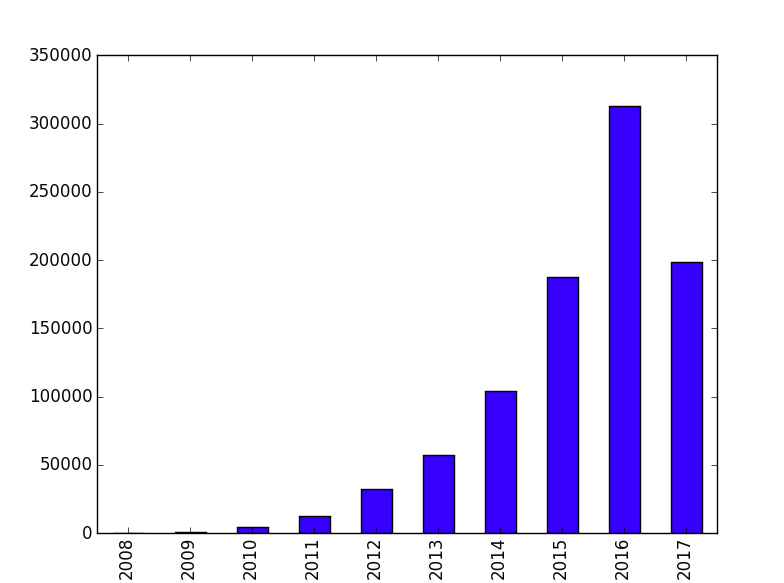
\includegraphics[width=\linewidth]{fig/fig1.png}
    \end{figure}

    La deuxième étape de l’étude s’intéresse à la place de l’environnement dans la communication des utilisateurs étudiés. Parmi les 1 110 utilisateurs qui composent le panel, 136 ont une mission liée à l’environnement. Toutefois, 763 utilisateurs ont publié au moins un tweet relatif à l’environnement, et 283 en ont publié au moins 10. La répartition en fonction des catégories d’organisations est présentée dans le Tableau \ref{table:15catenvir}. Les entreprises dont la mission est liée à la protection de l’environnement sont fortement représentées parmi les entreprises sociales. Cette partie émergente de l’ESS semble donc accorder un fort intérêt à ce secteur d’activité. A l’inverse, et de façon assez attendue, aucune mutuelle ni aucun organisme représentatif de l’ESS n’a une une activité environnementale. L’activité des mutuelles est réglementée et principalement tournée vers l’assurance et la santé. Le rôle des organismes représentatifs de l’ESS est de porter la voix de l’ensemble du secteur, dans toute la diversité de ses métiers. \\

    \begin{table}
    \caption{Dimension environnementale par type de compte }
    \label{table:15catenvir}
    \footnotesize

        \begin{tabularx}{\linewidth}{|X|r|r|r|r|r|r|}
        \hline
        \multirow{2}{*}{\textbf{Catégorie}} &	Comptes&	\multicolumn{2}{|X|}{\textbf{Comptes environnementaux}}	&
        Tweets&
        \multicolumn{2}{|X|}{\textbf{Tweets relatifs à l’environnement}} \\ \cline{2-7}
        &(Nombre)&\textbf{(Nombre)}&	\textbf{(\%)}
        &(Nombre*)&\textbf{(Nombre)}	&\textbf{(\% Moyen)} \\ \hline

        Association	&590&	80&	13.56&	522499&	13220&2.42 \\ \hline
        Autre	&26&	2&	7.69&	27439 &330	&1.65 \\ \hline
        Coopérative	&211&	21	&9.95&	129558& 2839&	2.35 \\ \hline
        Entreprise sociale	&75&	20&	26.67&	52135&2631&	5.55 \\ \hline
        Fondation	&115&	13&	11.30&	103268 & 3479&	2.53 \\ \hline
        Mutuelle	&67&	0&	0&	55998&475	&0.82 \\ \hline
        Fédérations - Organisme repr. & 26 &0 &0 &16896&247&1.35 \\ \hline
        \textbf{Total} &	\textbf{1110} &	\textbf{136} &	\textbf{12,25} &	\textbf{907793} &	\textbf{23221}& \\ \hline

        \end{tabularx}
        *Après exclusion des tweets répétés
    \end{table}




    Pour comparer les différents types d’entreprises indépendamment de leur activité environnementale ou non, nous nous intéressons au pourcentage de tweets ayant trait à l’environnement pour les organisations n’ayant pas une activité environnementale. Les données sont présentées dans le Tableau \ref{table:dimenenvirtypecomptenonenvir}. Exclusion faite des entreprises environnementales, le discours sur l’écologie est porté en premier lieu par les entreprises sociales (2,24 \% des tweets). Les coopératives et les utilisateurs de la catégorie « autre » consacrent plus de 1,5 \% de leurs publications aux sujets environnementaux. A l’opposé, les associations et mutuelles ont moins de 1 \% de tweets traitant des enjeux écologiques. \\


    \begin{table}
    \caption{Dimension environnementale des organisations non environnementales}
    \label{table:dimenenvirtypecomptenonenvir}
    \footnotesize

        \begin{tabularx}{\linewidth}{|X|r|r|r|r|r|r|}
        \hline

        \multirow{2}{*}{\textbf{Catégorie}}
        &\textbf{Comptes}
        &\textbf{Tweets}
        &\multicolumn{2}{|X|}{\textbf{Tweets environnementaux}} \\ \cline{2-5}

        &\textbf{(Nombre)}
        &\textbf{(Nombre)}
        &\textbf{(Nombre)}
        &\textbf{(\% moyen)} \\ \hline

       Entreprise sociale &	55 &	39 560 &	808 &	2,24 \\ \hline
        Coopérative	& 190 &	115 320 &	1 578 &	1,57 \\ \hline
        Autre	& 24 &	25 541 &	273 &	1,51 \\ \hline
        Fédérations - Organisme repr.	& 26 &	16 896	&247	&1,35 \\ \hline
        Fondation	& 102 &	85 876 &	912&	1,15 \\ \hline
        Association	& 510 &	448 951&	4 735&	0,94 \\ \hline
        Mutuelle	& 67 &	55 998&	475&	0,82 \\ \hline

        \textbf{Total} &	\textbf{974} &	\textbf{788142} &	\textbf{9028} &	\textbf{} \\ \hline

        \end{tabularx}
    \end{table}

    Dans cette étude, nous nous intéressons à la structure du réseau des acteurs de l’ESS sur Twitter, puis nous étudions les tweets à caractère environnemental selon l’approche de l’exploration de données.

\section{Analyse générale du corpus}
    \subsection{Etude des communautés}

        Dans un premier temps, on s’intéresse à la constitution en réseau des \oess. La figure \ref{figure:reseaumentions} permet de visualiser les communautés constituées par les liens entre les utilisateurs. Sur cette carte, les nœuds (cercles) correspondent aux comptes d’utilisateurs, et les liens qui relient deux utilisateurs indiquent que l’un a été mentionné par l’autre dans un tweet. La taille des nœuds est liée au degré entrant, c’est à dire au nombre de fois où l’utilisateur a été mentionné par un autre compte. Un compte recevant beaucoup de mentions joue un rôle central dans sa communauté.

        \begin{figure}
            \caption{Visualisation des liens inter-entreprises (basée sur les mentions)}
            \label{figure:reseaumentions}
            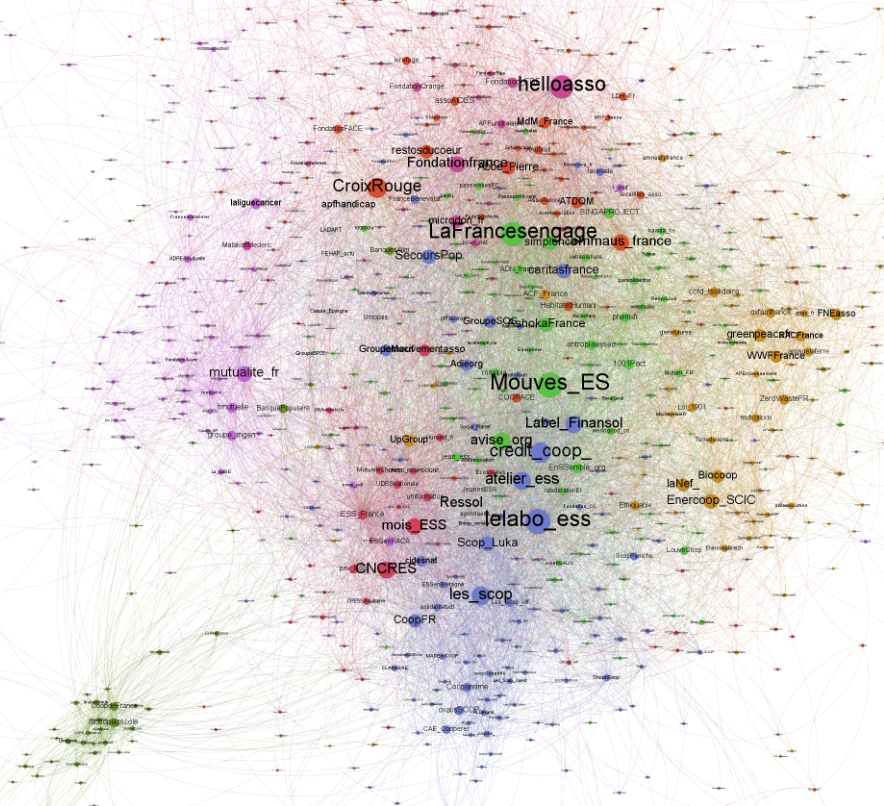
\includegraphics[width = \linewidth]{fig/fig2.png}
        \end{figure}

        Plusieurs communautés peuvent être mises en évidence. En bas à gauche (en vert), un groupe très distinct s’organise autour de Coop de France et la Coop Agricole (deux fédérations de coopératives agricoles). Autour, gravitent logiquement des coopératives agricoles, qui semblent former un réseau à part du reste de l’ESS.
        A gauche, en violet, un ensemble d’organisations s’organisent autour du compte de la Mutualité Française. Il s’agit essentiellement de mutuelles, mais aussi de fondations ou d’associations opérant dans le secteur de la santé, comme la Ligue Cancer et la Fondation de l’Avenir. Cette communauté se détache légèrement du reste de l’ESS mais laisse toutefois apparaître de nombreux liens avec d’autres groupes.
        En haut de la carte, deux communautés (en rouge et en rose) apparaissent très interconnectées. Il s’agit essentiellement de fondations et d’associations caritatives, organisées autour de l’entreprise HelloAsso (dont la mission est le financement de projets associatifs), de la Fondation de France (principale Fondation abritante en France) et d’entreprises symboliques du secteur non lucratif comme la Fondation Abbé Pierre, les Restos du Cœur, Emmaüs France, ou encore la Croix Rouge). Cette double communauté correspond donc au secteur de l’action sociale et de la solidarité.
        Sur la partie droite de la carte, en orange, une communauté se forme autour de la thématique de l’action environnementale. Deux sous-groupes se distinguent : le premier (en haut) autour de Green Peace, WWF France et France Nature Environnement ; le second autour de Enercoop (fournisseur d’énergie issue de sources renouvelables), Biocoop (épiceries bio) et la Nef (coopérative bancaire). Le premier groupe correspond à une action directe pour protéger l’environnement, quand le second propose des modes de consommation alternatifs pour limiter l’impact sur l’environnement.
        En bas de la carte (en bleu), des entreprises essentiellement coopératives s’organisent autour d’organismes de fédération et de promotion de l’ESS comme Le Labo ESS, Le mouvement des SCOP, Coop FR (qui anime le mouvement coopératif en France) ou encore l’Atelier ESS. Cette communauté est là aussi très interconnectée avec celle qui se trouve à sa gauche (rouge clair), qui fait apparaître d’autres instances représentatives comme le CNCRES, le Mois ESS, et ESS France (organisme institué par la loi ESS de 2014).
        Enfin, une communauté apparaît en position centrale, avec notamment de fortes interactions avec la communauté caritative, la communauté coopérative et la communauté environnementale. Elle s’organise autour d’organisations phares de l’entrepreneuriat social comme le \mouves, La France s’engage (label qui encourage les projets innovants), Ashoka France (association de promotion des entreprises sociales) et Avise (portail du développement de l’ESS). Il est intéressant de constater que cette communauté maintient des liens étroits avec trois groupes qui se distinguent nettement les uns des autres (le secteur caritatif, le secteur environnemental et le secteur coopératif). Ceci illustre le positionnement de l’entrepreneuriat social qui s’intéresse à tous les secteurs de l’ESS, mais se différencie plutôt par une démarche caractérisée par une démarche gestionnaire codifiée (avec notamment une grande proximité avec le milieu des startups), et un fort accent mis sur l’innovation. \\

        Une disposition similaire est observée avec une approche différente, dans laquelle les liens ne correspondent plus aux mentions mais aux abonnements (figure \ref{figure:reseauabos}). Ces liens sont pondérés. Pour deux utilisateurs A et B, le lien entre les deux a une valeur de 1 si A est abonné à B mais B n’est pas abonné à A, et une valeur de 2 si A et B sont mutuellement abonnés. Le fait de s’abonner à un utilisateur représente une action plus passive, puisqu’elle ne nécessite pas d’interaction : on indique simplement que l’on souhaite être informé des publications d’un utilisateur. C’est donc davantage un lien d’intérêt mutuel ou à sens unique.

        \begin{figure}
            \caption{Visualisation des liens inter-entreprises (basée sur les abonnements)}
            \label{figure:reseauabos}
            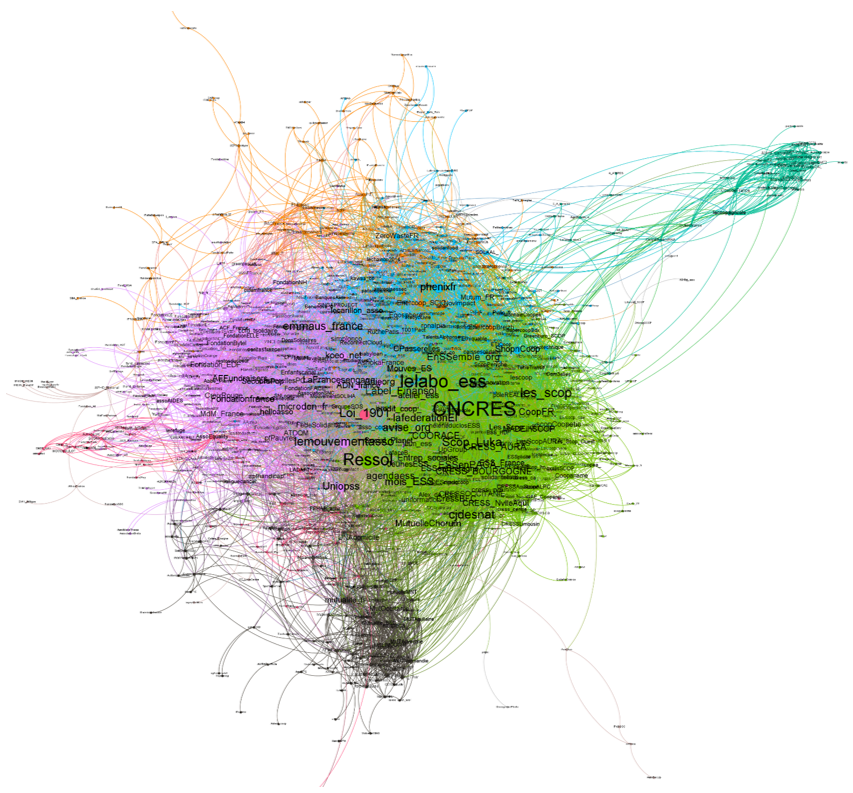
\includegraphics[width = \linewidth]{fig/fig3.png}
        \end{figure}

        La communauté des coopératives agricoles (en haut à droite) apparaît à nouveau très isolée du reste des utilisateurs qui forme un ensemble très interconnecté. Les mutuelles apparaissent en bas, formant également une communauté très homogène. Deux communautés majeures adoptent une position centrale sur la figure : la première (à droite, en vert) regroupe les organes de représentation de l’ESS, avec notamment le CNCRES, les CRESS et le Labo ESS. Le mouvement coopératif est intégré à cette communauté. A gauche, en violet, on retrouve la communauté ‘caritative’, qui regroupe fondations et associations ayant une forte mission sociale. Un sous-groupe de cette communauté se distingue à gauche : il s’agit d’organisations de lutte pour la tolérance et de défense des minorités, en particulier LGBT. Au-dessus, en bleu, la communauté des entrepreneurs sociaux, avec notamment de nombreuses startups assez jeunes (1001pact, Mutum, ShopnCoop, Pwiic…), semble à nouveau très ouverte, très connectée avec les autres groupes. La communauté ‘environnementale’ (en orange, en haut) se distingue moins nettement et tend à se confondre avec la communauté des entreprises sociales.

    \subsection{Statistiques multivariées}
        Afin de garantir la validité des résultats des deux régressions effectuées et de permettre la généralisation à une population, un certain nombre de critères doivent être respectés \parencite{field2009discovering}.
        Les variables explicatives de la régression sont continues, à l’exception de la variable ‘catégorie’ qui est catégorielle. Leur variance est non nulle. Toutes les valeurs de la variable expliquée sont indépendantes (chaque valeur correspond à un compte Twitter différent : c’est la raison pour laquelle le choix a été fait de ne considérer chaque compte qu’une seule fois en agrégeant les données de la période d’étude). La matrice des corrélations (tableau \ref{table:12correlations}) permet de vérifier l’absence de multicolinéarité parfaite. Le seul point d’attention relevé par ce test est la corrélation relativement importante entre le nombre de tweets avec mentions et le nombre de tweets avec un hashtag, qui invite à une interprétation prudente des coefficients correspondants. Les critères d’homoscédasticité et de distribution normale du terme d’erreur sont vérifiés visuellement grâce à la figure \ref{figure:5residus}. La distribution du terme d’erreur suit bien la structure d’une loi normale et la variance du test d’erreur ne dépend pas de la valeur prédite. Le résultat du test de Durbin-Watson est compris entre 1 et 3 et proche de 2 pour les deux modèles, ce qui garantit l’indépendance des termes résiduels. Enfin, les nuages de points confrontant les différentes variables du modèle suggèrent bien l’existence d’une relation linéaire qui justifie le recours à un modèle linéaire. Ainsi, le modèle semble donc approprié et généralisable à la population.

        \begin{landscape}

            \begin{table}
            \renewcommand{\arraystretch}{1.5}
            \begin{footnotesize}
                \caption{Matrice des corrélations}
                \label{table:12correlations}
                \begin{tabularx}{\linewidth}{|p{2cm}|X|X|X|X|X|X|X|X|X|}
                \hline
                &&\textbf{Nb\_ retweeted}&	\textbf{Nb\_ tw\_ hashtags}	&\textbf{nb\_ abonnements}	&\textbf{nb\_ abonnes}&	\textbf{nb\_ favoris}	&\textbf{nb\_ mentions}	&\textbf{nb\_ reponses}	&\textbf{nb\_ tweets}
                \\ \hline
                \multirow{2}{=}{\textbf{Nb\_ retweeted}}
                    &corr&1.000***&	0.400***&	0.121***&	0.699***&	0.879***&	0.291***&	0.171***&	0.291***\\
                    \cline{2-10}
                    &p-value&(0.000)&	(0.000)	&(0.000)&	(0.000)&	(0.000)	&(0.000)&	(0.000)&	(0.000)
                    \\ \hline
                \multirow{2}{=}{\textbf{Nb\_tw\_ hashtags}}
                    &corr&0.400***&	1.000***&	0.245***&	0.255***&	0.374***&	0.762***&	0.359***&	0.332***\\
                    \cline{2-10}
                    &p-value&(0.000)&	(0.000)	&(0.000)&	(0.000)	&(0.000)&	(0.000)	&(0.000)&	(0.000)
                    \\ \hline
                \multirow{2}{=}{\textbf{nb\_ abonnements}}
                    &corr&0.121***&	0.245***&	1.000***	&0.113***&	0.110***&	0.248***&	0.145***&	0.238***\\
                    \cline{2-10}
                    &p-value&	(0.000)&	(0.000)	&(0.000)	&(0.000)&	(0.000)&	(0.000)	&(0.000)&	(0.000)
                    \\ \hline
                \multirow{2}{=}{\textbf{nb\_abonnes}}
                    &corr&0.699***&	0.255***&	0.113***&	1.000***&	0.808***&	0.180***&	0.157***&	0.243***\\
                    \cline{2-10}
                    &p-value&(0.000)&	(0.000)	&(0.000)&	(0.000)&	(0.000)&	(0.000)&	(0.000)	&(0.000)
                    \\ \hline
                \multirow{2}{=}{\textbf{nb\_favoris}}
                    &corr&0.879***&	0.374***&	0.110***&	0.808***&	1.000***&	0.272***&	0.164***&	0.297***\\
                    \cline{2-10}
                    &p-value&(0.000)&	(0.000)&	(0.000)	&(0.000)&	(0.000)	&(0.000)&	(0.000)&	(0.000)
                    \\ \hline
                \multirow{2}{=}{\textbf{nb\_ mentions}}
                    &corr&0.291***&	0.762***&	0.248***&	0.180***&	0.272***&	1.000***&	0.699***&	0.356***\\
                    \cline{2-10}
                    &p-value&(0.000)&	(0.000)	&(0.000)&	(0.000)&	(0.000)	&(0.000)&	(0.000)	&(0.000)
                    \\ \hline
                \multirow{2}{=}{\textbf{nb\_ reponses}}
                    &corr&0.171***&	0.359***&	0.145***	&0.157***	&0.164***&	0.699***&	1.000***&	0.262***\\
                    \cline{2-10}
                    &p-value&(0.000)	&(0.000)&	(0.000)	&(0.000)&	(0.000)	&(0.000)&	(0.000)	&(0.000)
                    \\ \hline
                \multirow{2}{=}{\textbf{nb\_ tweets}}
                    &corr&0.291***&	0.332***&	0.238***&	0.243***&	0.297***&	0.356***&	0.262***&	1.000*** \\
                    \cline{2-10}
                    &p-value&(0.000)&	(0.000)	&(0.000)&	(0.000)	&(0.000)&	(0.000)	&(0.000)&	(0.000)
                    \\ \hline

                \end{tabularx}
            \end{footnotesize}
            \end{table}
        \end{landscape}


        \begin{landscape}
        \begin{figure}
            \caption{Hétéroscédasticité et normalité des résidus}
            \label{figure:5residus}
            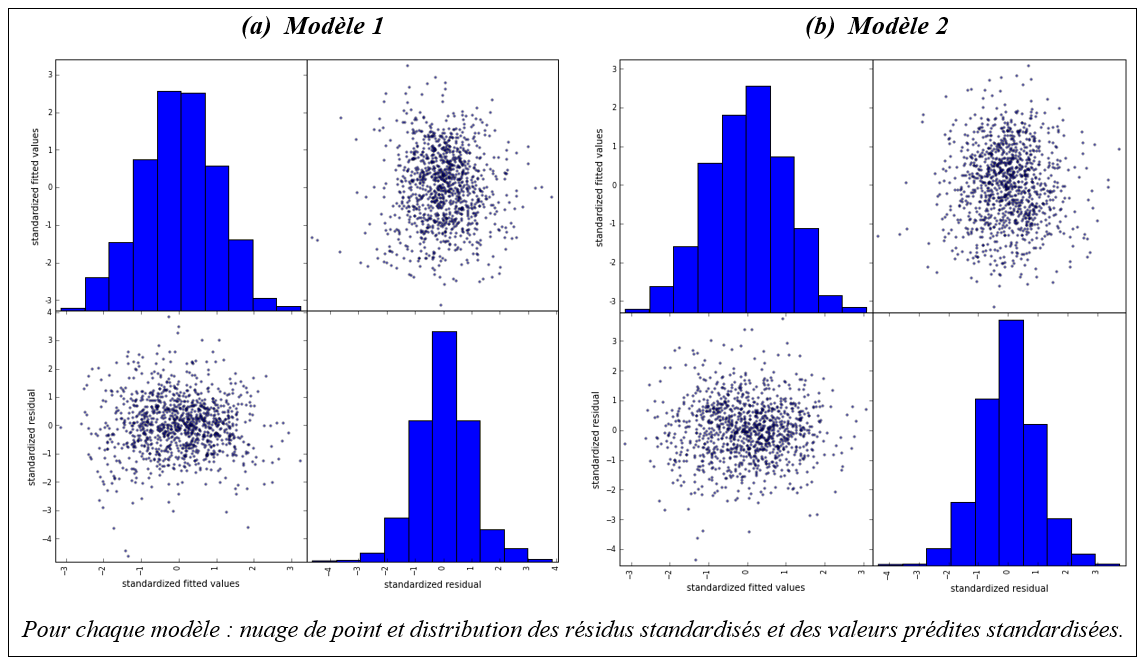
\includegraphics[width = \linewidth]{fig/fig5.PNG}
        \end{figure}
        \end{landscape}


        \begin{table}
        \caption{Résultats de la régression - modèle 1}
        \label{table:13regress1}
            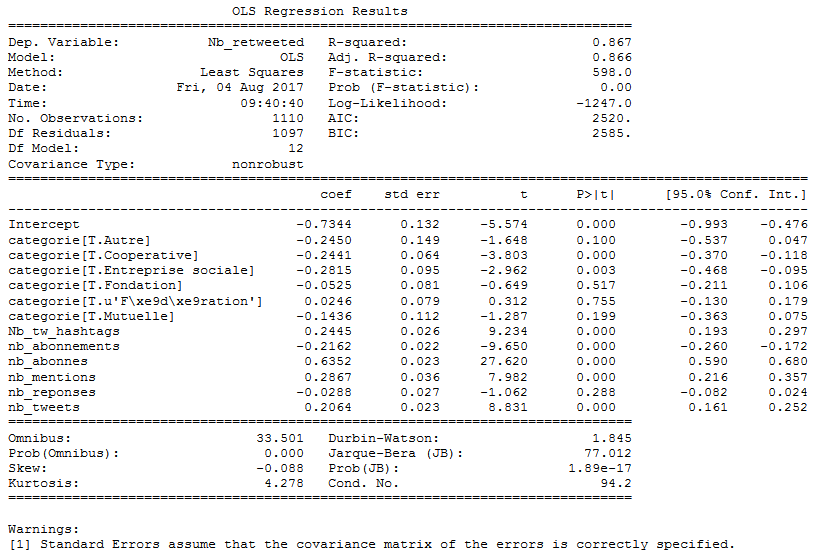
\includegraphics[width = \linewidth]{fig/tbl_regress1.png}
        \end{table}

        \begin{table}
        \caption{Résultats de la régression - modèle 2}
        \label{table:13regress2}
            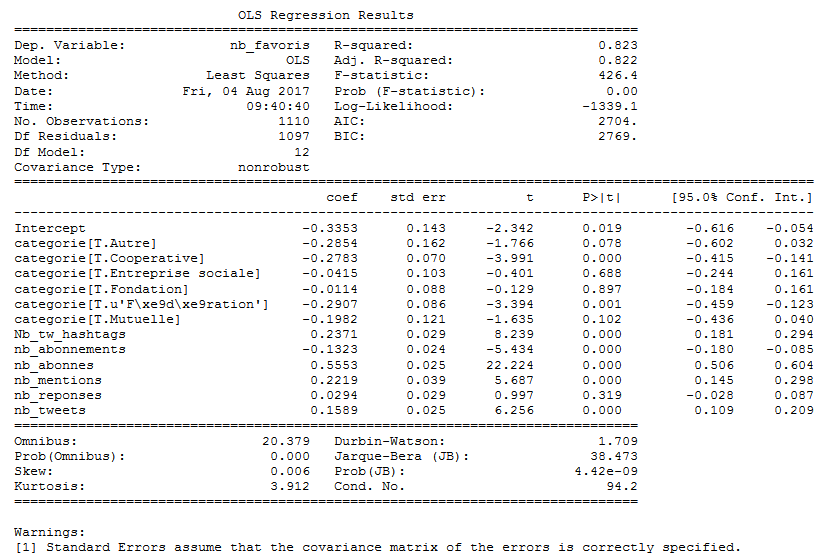
\includegraphics[width = \linewidth]{fig/tbl_regress2.png}
        \end{table}


        Les deux modèles (tableau \ref{table:13regress1} pour le nombre de retweets et \ref{table:13regress2} pour le nombre de favoris) présentent un fit ($R^2$) supérieur à 0.8 et sont donc très satisfaisants. Ils convergent globalement avec les résultats de Guo et Saxton. Tout d’abord, les résultats montrent que le niveau d’attention d’un compte est positivement associé au nombre d’abonnés, aussi bien pour le nombre de retweets que le nombre de favoris. Les coefficients associés (0.64 et 0.56 resp.) soulignent l’importance de cette donnée dans l’attention reçue par un compte. Le nombre de tweets publiés est un facteur relativement moins important, mais néanmoins très significatif de l’attention reçue. Le nombre de réponses faites à d’autres utilisateurs impacte positivement le nombre de favoris, mais négativement le nombre de retweets. Cependant, ce résultat est à prendre avec précautions, car les intervalles de confiance de 95\% prennent à la fois des valeurs positives et négatives pour les deux modèles. En réalité, l’influence du nombre de réponses est significative, mais très proche de zéro et n’est donc pas déterminante. En revanche, le nombre de tweets incluant au moins un hashtag impacte positivement le nombre de retweets et le nombre de favoris obtenus par un compte. Contrairement à Guo et Saxton, les deux modèles suggèrent qu’il existe bien un impact positif du nombre de tweets mentionnant un autre utilisateur sur l’attention obtenue. Par ailleurs, l’étude apporte un nouveau résultat intéressant : le nombre d’abonnements est négativement lié à l’attention obtenue. Enfin, de façon assez imprévisible, le fait d’être une coopérative a un impact négatif sur l’attention reçue pour les deux indicateurs. Appartenir au groupe des entreprises sociales impacte aussi négativement le nombre de retweet, et à celui des fédérations réduit le nombre de favoris.


    \subsection{Place du discours environnemental}

        Parmi les 1 110 utilisateurs qui composent le panel, 136 ont une mission liée à l’environnement. Toutefois, 763 utilisateurs ont publié au moins un tweet relatif à l’environnement et le nombre total de tweets environnementaux s’élève à 23 221. La répartition en fonction des catégories d’organisations est présentée dans le tableau \ref{table:15catenvir}.

        % \begin{table}
        % \caption{Catégorie de comptes et dimension environnementale }
        % \label{table:15catenvir}
        % \footnotesize

        %     \begin{tabularx}{\linewidth}{|l|r|r|r|r|r|}
        %     \hline
        %     \multirow{2}{*}{\textbf{Catégorie}} &	\multirow{2}{*}{\textbf{Effectif total}} &	\multicolumn{2}{|X|}{\textbf{Organisations environnementales}}	& \multicolumn{2}{|X|}{\textbf{Tweets relatifs à l’environnement}} \\ \cline{3-6}
        %     &&\textbf{Nombre}&	\textbf{Pourcentage}	&\textbf{Nombre}	&\textbf{Pourcentage} \\ \hline

        %     Association	&544&	69&	12,68&	12666&	2.27 \\ \hline
        %     Coopérative	&191&	21	&10,99&	2558&	2.28 \\ \hline
        %     Entreprise sociale	&73&	20&	27,40&	2573&	6.34 \\ \hline
        %     Fondation	&114&	13&	11,40&	3399&	1.87 \\ \hline
        %     Fédération	&111&	9&	8,11&	2935&	3.48 \\ \hline
        %     Autre	&27&	4&	14,81&	467	&2.23 \\ \hline
        %     Mutuelle	&50&	0&	0&	290	&0.55 \\ \hline
        %     \textbf{Total} &	\textbf{1110} &	\textbf{136} &	\textbf{12,36} &	\textbf{24888} &	\textbf{2.73} \\ \hline

        %     \end{tabularx}

        % \end{table}

        \subsubsection{Lien entre activité environnementale et discours environnemental}
        Bien que les organisations environnementales ne soient pas les seules à publier des tweets en lien avec ces questions, il est très probable qu’elles adoptent un discours plus fortement lié à l’environnement. Pour le vérifier, nous comparons le pourcentage de tweets relatifs à l’environnement entre deux groupes : les utilisateurs dont l’activité concerne l’environnement et ceux dont l’activité est hors secteur environnemental. On étudie la variable Pc\_envir qui correspond au pourcentage de tweets concernant l’environnement pour chaque utilisateur. La normalité de cette variable est testée à l’aide du test de Shapiro-Wilk et du test de Kolmogorov-Smirnov. Comme le montre le tableau \ref{table:16normalite}, les résultats sont fortement significatifs et l’hypothèse de normalité est donc rejetée. \\


        \begin{table}
        \caption{Test de normalité de la variable Pc\_envir}
        \label{table:16normalite}
        \footnotesize

            \begin{tabularx}{\linewidth}{|K{2cm}|K{4cm}|C|C|C|C|}
            \hline
            \multicolumn{2}{|c|}{}&	\multicolumn{2}{c|}{\textbf{Shapiro-Wilk}} &	\multicolumn{2}{c|}{\textbf{Kolmogorov-Smirnov}}\\ \cline{3-6}
            \multicolumn{2}{|c|}{}&\textbf{Stat}&	\textbf{p-value}	&\textbf{stat}	&\textbf{p-value} \\ \hline

            \multirow{3}{*}{Pc\_envir}
                &Ensemble des entreprises &	0.885 &	0.000 &	0.500 &	0.0\\ \cline{2-6}
                &Activité non liée à l’environnement &	0.876 &	0.000 &	0.500 &	0.0\\ \cline{2-6}
                &Activité liée à l’environnement &	0.966 &	0.002 &	0.529 &	0.0\\ \hline


            \end{tabularx}

        \end{table}

        Pour comparer les deux groupes, un test non paramétrique est donc utilisé : celui de Wilcoxon. Ce test repose sur un classement des individus du panel en fonction du classement des données, et non en fonction des données elles-mêmes : par conséquent il ne dépend pas de la distribution des variables étudiées \parencite{field2009discovering}. L’application du test nécessite de comparer deux échantillons de même taille, or l’échantillon n’est pas équitablement réparti entre les deux groupes. Le test est donc réalisé sur une sélection aléatoire de 100 individus au sein de chaque groupe. Le résultat est significatif au seuil de 1\% (tableau \ref{table:16wilcoxon}).

        \begin{table}
        \centering
        \caption{Résultats du test de Wilcoxon}
        \label{table:16wilcoxon}
            \begin{tabular}{|l|c|c|}
            \hline
            &\multicolumn{2}{|c|}{Wilcoxon} \\ \cline{2-3}
            & Stat & p-value \\ \hline
            Variable Pc\_envir & 253.0	& 0.000 \\ \hline
            \end{tabular}
        \end{table}

        Le test est renouvelé à plusieurs reprises avec un sous-échantillon différent et aboutit toujours à un résultat similaire. Comme escompté, les entreprises dont l’activité est liée à l’environnement ont donc un discours plus orienté vers les questions qui s’y rattachent que les entreprises dont le métier ne concerne pas l’écologie .



        \subsubsection{Lien entre type de compte d’utilisateur et discours environnemental}
        Comme le montre le tableau \ref{table:15catenvir}, les entreprises environnementales sont principalement représentées parmi les entreprises sociales et au sein de la catégorie ‘autre’. Au contraire, parmi les mutuelles, aucune n’est dédiée à l’environnement, leur secteur d’activité étant légalement restreint à l’assurance et la santé. \\

        Une comparaison de la proportion de tweets à caractère environnemental entre les différentes catégories peut être effectuée. Là encore, en raison de la non-normalité des variables, un test non-paramétrique, celui de Kruskal-Wallis est réalisé. Son fonctionnement est similaire à celui de Wilcoxon, mais généralisable à plus de deux groupes. Quel que soit le critère retenu, le test est significatif au seuil de 5\% suggérant qu’au moins l’une des catégories a un pourcentage de tweet relatifs à l’environnement significativement différent des autres (tableau \ref{table:17KW}). Pour déterminer laquelle, on effectue des comparaisons deux à deux entre les 8 groupes, ce qui nous conduit à effectuer 28 tests. \\


        \begin{table}
        \centering
        \caption{Résultats du test de Kruskal-Wallis}
        \label{table:17KW}
            \begin{tabular}{|l|c|c|}
            \hline
            &\multicolumn{2}{|c|}{Wilcoxon} \\ \cline{2-3}
            & Stat H & p-value \\ \hline
            Pc\_envir\_crit1	& 33.2416	& 0.000\\ \hline
            Pc\_envir\_crit2	& 55.4461	& 0.000\\ \hline
            Pc\_envir\_crit3	& 57.4710	& 0.000\\ \hline

            \end{tabular}
        \end{table}


        Conformément à ce qui est recommandé par \textcite{field2009discovering}, le test de Mann-Whitney est utilisé pour ces comparaisons deux à deux et la correction de Bonferoni est appliquée afin de limiter le taux d’erreur de Type 1. Ainsi, on évalue la qualité du test en divisant la valeur critique par le nombre de tests réalisés. Par conséquent, les résultats seront jugés significatifs au seuil de 5\% si la p-value est inférieure à 0.05/21 et au seuil de 1\% si la p-value est inférieure à 0.01/21. Les résultats présentés dans le tableau \ref{table:19MW} prennent en compte cette correction. \\

        \begin{table}
            \caption{Résultats des tests de Mann-Whitney – tous comptes d’utilisateurs}
            \label{table:19MW}
            \scriptsize

            \begin{tabularx}{\linewidth}{|l|K{0.4cm}|L|L|L|L|L|L|L|}
            \hline
            &&Association	& Autre	& Coopérative	& Entreprise Sociale	& Fondation& 	Fédération	& Mutuelle \\ \hline

            Association	&U&	147968&	5530&	45371&	12108***&	28299&	22515***&	11835 \\
        	    &P	&(0.5000)&	(0.0131)&	(0.0038)&	(0.0000)&	(0.0663)&	(0.0000)&	(0.0589)\\ \hline

            Autre&	U&	5530&	364&	2313&	790&	1222&	1493&	379\\
            	&P&	(0.0131)	&(0.4965)&	(0.1903)&	(0.0645)&	(0.0470)&	(0.4893)&	(0.0006)\\ \hline

            Coopérative&	U&	45371&	2313&	18240&	4992**	&10168	&9404	&3430\\
            	&P&	(0.0038)&	(0.1903)&	(0.4998)&	(0.0002)&	(0.1640)&	(0.0494)&	(0.0009)\\ \hline

            Entreprise Sociale&	U&	12108***&	790&	4992**&	2664	&2662***&	3272&	798***\\
            &	P&	(0.0000)&	(0.0645)&	(0.0002)&	(0.4992)&	(0.0000)&	(0.0136)&	(0.0000)\\ \hline

            Fondation&	U&	28299&	1222&	10168&	2662***	&6498&	5031&	2190\\
            &	P&	(0.0663)&	(0.0470)&	(0.1640)&	(0.0000)&	(0.4996)&	(0.0038)&	(0.0082)\\ \hline

            Fédération - Org. Repr.&	U&	22515***&	1493&	9404&	3272&	5031&	6160&	1570***\\
            &	P&	(0.0000)&	(0.4893)&	(0.0494)&	(0.0136)&	(0.0038)&	(0.4996)&	(0.0000)\\ \hline

            Mutuelle&	U&	11835&	379&	3430&	798***&	2190&	1570***&	1250\\
            &	P&	(0.0589)&	(0.0006)&	(0.0009)&	(0.0000)&	(0.0082)&	(0.0000)&	(0.4980)\\ \hline

            \end{tabularx}
        \end{table}

        \begin{table}
            \caption{Résultats des tests de Mann-Whitney – hors organisations environnementales}
            \label{table:20MWbis}
            \scriptsize

            \begin{tabularx}{\linewidth}{|l|K{0.4cm}|L|L|L|L|L|L|L|}
            \hline
            &&Association	& Autre	& Coopérative	& Entreprise Sociale	& Fondation& 	Fédération	& Mutuelle \\ \hline


                Association			&U&	112812	&   	3806	&	33136**	&	7029***	&	20738	&	16115***&	11687\\
                					&p&	(0.5000)&   	(0.0053)&	(0.0002)&	(0.0000)&	(0.0133)&	(0.0000)&	(0.4240)\\ \hline
                Autre				&U&	3806	&   	264	&       1750&		511		&	916		&	1149	&	375     \\
                					&p&	(0.0053)&   	(0.4956)&	(0.2027)&	(0.1330)&	(0.0550)&	(0.4402)&	(0.0074)\\ \hline
                Coopérative			&U&	33136**	&   	1750	&	14450	&	3324	&	7926	&	7518	&	3346\\
                					&p&	(0.0002)&   	(0.2027)&	(0.4998)&	(0.0017)&	(0.1408)&	(0.0315)&	(0.0095)\\ \hline
                Entreprise Sociale	&U&	7029***	&   	511		&	3324	&	1404	&	1705**	&	2296	&	672***\\
                					&p&	(0.0000)&   	(0.1330)&	(0.0017)&	(0.4987)&	(0.0001)&	(0.0616)&	(0.0000)\\ \hline
                Fondation			&U&	20738	&   	916		&	7926	&	1705**	&	5100	&	3900	&	2146\\
                					&p&	(0.0133)&   	(0.0550)&	(0.1408)&	(0.0001)&	(0.4995)&	(0.0013)&	(0.0628)\\ \hline
                Fédération - Org. repr.			&U&	16115***&   	1149	&	7518	&	2296	&	3900	&	5202	&	1567**\\
                					&p&	(0.0000)&   	(0.4402)&	(0.0315)&	(0.0616)&	(0.0013)&	(0.4995)&	(0.0000)\\ \hline
                Mutuelle			&U&	11687	&   	375		&	3346	&	672***	&	2146	&	1567**	&	1250\\
                					&p&	(0.4240)&   	(0.0074)&	(0.0095)&	(0.0000)&	(0.0628)&	(0.0000)&	(0.4986)\\ \hline


            \end{tabularx}
        \end{table}


        Ces tests montrent que les entreprises sociales consacrent un pourcentage de tweets à l’environnement significativement plus élevé que les associations, fondations et mutuelles (seuil de 1\%) et que les coopératives (seuil de 5\%). A l’opposé, les associations et mutuelles publient moins de tweets relatifs à l’environnement que les fédérations. Toutefois, ce résultat peut être influencé par la proportion importante d’entreprises sociales qui ont une activité environnementale et qui donc publient davantage de tweets relatifs à l’écologie. Inversement, les associations environnementales sont « noyées » dans une masse d’organisations ayant des missions différentes. Pour neutraliser cet impact, les tests sont reproduits sur l’échantillon après élimination des utilisateurs liés à l’environnement (N = 974). Les résultats sont très similaires, voire plus significatifs (tableau \ref{table:20MWbis}). La différence est particulièrement marquée entre d’un côté les coopératives et entreprises sociales, et de l’autre les associations. Les entreprises sociales publient aussi davantage de tweets concernant l’environnement que les fondations et mutuelles. Le discours environnemental semble donc plutôt adopté par des entreprises de l’ESS ayant des caractéristiques proches des entreprises classiques .

\section{Exploration de texte}
    \subsection{Extraction des thématiques principales}
        Trois algorithmes sont utilisés pour faire émerger des catégories thématiques à partir des mots du corpus. L’algorithme NMF avec la norme de Frobenius donne les meilleurs résultats. Six thématiques sont mises en évidence (pour n=5, les catégories sont peu lisibles ; à partir de n=7, des catégories non porteuses de sens apparaissent). Les éléments les plus significatifs sont présentés dans le Tableau \ref{table:thematiquesemergentes}.

        \begin{scriptsize}
        \renewcommand*{\arraystretch}{0.8}
        \begin{longtable}{
            |>{\setlength{\baselineskip}{0.7\baselineskip}}K{0.14\textwidth}
            |>{\setlength{\baselineskip}{0.7\baselineskip}}K{0.14\textwidth}
            |>{\setlength{\baselineskip}{0.7\baselineskip}}K{0.14\textwidth}
            |>{\setlength{\baselineskip}{0.7\baselineskip}}K{0.14\textwidth}
            |>{\setlength{\baselineskip}{0.7\baselineskip}}K{0.14\textwidth}
            |>{\setlength{\baselineskip}{0.7\baselineskip}}K{0.14\textwidth}
            | }
            \caption{Thématiques émergentes}
            \label{table:thematiquesemergentes} \\ \hline

            1 - Climat	&	2 - Pollution	&	3 - Recyclage	&	4 - Agriculture 	&	5 - Energie	&	6 - Biodiversité	\\ \hline
            \endfirsthead \hline
            1 - Climat	&	2 - Pollution	&	3 - Recyclage	&	4 - Agriculture 	&	5 - Energie	&	6 - Biodiversité	\\
            \multicolumn{6}{|c|}{(Suite)} \\ \hline
            \endhead

            \cellcolor{blue!25}climat (6.72)	&	\cellcolor{blue!25}pollution (4.99)	&	\cellcolor{blue!25}recyclage (3.28)	&	\cellcolor{blue!25}bio (6.01)	&	\cellcolor{blue!25}énergie (6.19)	&	\cellcolor{blue!25}biodiversité (5.86)	\\

            \cellcolor{blue!25}cop21 (3.76)	&	\cellcolor{blue!25}air (2.95)	&	\cellcolor{blue!25}economiecirculaire (2.55)	&	\cellcolor{blue!25}agriculture (1.74)	&	\cellcolor{blue!25}renouvelable (1.14)	&	\cellcolor{blue!25}loup (0.86)	\\

            \cellcolor{blue!25}climatique (0.89)	&	\cellcolor{blue!25}polluant (1.45)	&	\cellcolor{blue!25}déchets (2.28)	&	\cellcolor{blue!25}local (0.54)	&	\cellcolor{blue!25}nucléaire (0.82)	&	\cellcolor{blue!25}nature (0.85)	\\

            \cellcolor{blue!25}charbon (0.58)	&	\cellcolor{blue!25}iledefrance (1.43)	&	ess (2.24)	&	\cellcolor{blue!25}biologique (0.53)	&	économie (0.76)	&	\cellcolor{blue!25}anb2016 (0.71)	\\

            \cellcolor{blue!25}accord (0.53)	&	\cellcolor{blue!25}épisode (1.25)	&	projet (1.62)	&	\cellcolor{blue!25}alimentation (0.48)	&	\cellcolor{blue!25}enr (0.57)	&	\cellcolor{blue!25}canislupus (0.54)	\\

            \cellcolor{blue!25}changement (0.52)	&	pm10 (1.23)	&	durable (1.54)	&	\cellcolor{blue!25}pesticides (0.4)	&	\cellcolor{blue!25}enercoop (0.44)	&	\cellcolor{blue!25}ouiauxloups (0.5)	\\

            \cellcolor{blue!25}paris (0.51)	&	attention (1.13)	&	nouveau (1.36)	&	conférence (0.29)	&	\cellcolor{blue!25}solaire (0.44)	&	ateliercoecolo (0.44)	\\

            agir (0.39)	&	prévoir (1.13)	&	transition (1.35)	&	\cellcolor{blue!25}produit (0.28)	&	\cellcolor{blue!25}électricité (0.38)	&	loi (0.38)	\\
            pr (0.34)	&	santé (0.61)	&	social (1.32)	&	\cellcolor{blue!25}bon (0.27)	&	\cellcolor{blue!25}transitionenergetique (0.35)	&	agriculture (0.24)	\\
            devoir (0.34)	&	idf (0.49)	&	écolo (1.31)	&	\cellcolor{blue!25}manger (0.25)	&	positif (0.34)	&	royalsegolene (0.22)	\\
            tout (0.29)	&	\cellcolor{blue!25}episode (0.48)	&	découvrir (1.2)	&	\cellcolor{blue!25}biocoop (0.25)	&	france (0.33)	&	france (0.21)	\\
            mobilisation (0.28)	&	\cellcolor{blue!25}particule (0.43)	&	merci (1.08)	&	\cellcolor{blue!25}agroécologie (0.24)	&	citoyen (0.31)	&	français (0.19)	\\
            dire (0.27)	&	\cellcolor{blue!25}airparif (0.37)	&	\cellcolor{blue!25}zerowaste (0.81)	&	rdv (0.21)	&	\cellcolor{blue!25}fossile (0.31)	&	eau (0.18)	\\
            \cellcolor{blue!25}réchauffement (0.27)	&	constater (0.35)	&	dd (0.77)	&	découvrir (0.18)	&	\cellcolor{blue!25}énergétique (0.3)	&	agence (0.17)	\\
            santé (0.26)	&	\cellcolor{blue!25}qualité (0.28)	&	paris (0.76)	&	\cellcolor{blue!25}producteur (0.18)	&	\cellcolor{blue!25}consommation (0.29)	&	\cellcolor{blue!25}protection (0.17)	\\
            conférence (0.26)	&	\cellcolor{blue!25}paris (0.27)	&	france (0.75)	&	nouveau (0.18)	&	\cellcolor{blue!25}edf (0.23)	&	national (0.16)	\\
            engager (0.26)	&	\cellcolor{blue!25}atmosphérique (0.19)	&	énergétique (0.74)	&	coopérative (0.17)	&	damienhasbroucq (0.22)	&	\cellcolor{blue!25}chasse (0.14)	\\
            \cellcolor{blue!25}cop22 (0.26)	&	faible (0.18)	&	développement (0.74)	&	\cellcolor{blue!25}équitable (0.17)	&	promotelec (0.21)	&	note (0.13)	\\
            racfrance (0.26)	&	\cellcolor{blue!25}pic (0.18)	&	\cellcolor{blue!25}déchet (0.73)	&	petit (0.17)	&	\cellcolor{blue!25}energie (0.2)	&	préserver (0.12)	\\
            action (0.26)	&	lt (0.17)	&	\cellcolor{blue!25}ateliercoecolo (0.71)	&	semaine (0.15)	&	parler (0.2)	&	nouveau (0.12)	\\
            engagement (0.24)	&	savoir (0.17)	&	tout (0.68)	&	santé (0.15)	&	transition (0.19)	&	agir (0.11)	\\
            solution (0.23)	&	ville (0.15)	&	économie (0.61)	&	ligne (0.15)	&	\cellcolor{blue!25}renouvelables (0.18)	&	protéger (0.11)	\\
            monde (0.22)	&	france (0.14)	&	solidaire (0.61)	&	magasin (0.14)	&	\cellcolor{blue!25}transitionénergétique (0.18)	&	projet (0.11)	\\
            alimentation (0.21)	&	intérieur (0.14)	&	\cellcolor{blue!25}recycler (0.57)	&	cantine (0.14)	&	amorce (0.18)	&	\cellcolor{blue!25}biocentrisme (0.11)	\\
            pouvoir (0.2)	&	an (0.13)	&	parler (0.55)	&	solidaire (0.14)	&	vert (0.17)	&	sauver (0.1)	\\
            \cellcolor{blue!25}climatechange (0.2)	&	voiture (0.13)	&	citoyen (0.52)	&	tout (0.13)	&	europe (0.16)		& coprae (0.1)	\\
            agriculture (0.19)	&	fin (0.13)	&	entreprise (0.52)	&	beau (0.13)	&	logement (0.16)	&	merci (0.1)	\\
            nouaillas (0.19)	&	enfant (0.13)	&	soutenir (0.49)	&\cellcolor{blue!25}	filière (0.12)	&	grâce (0.16)	&	journée (0.09)	\\
            olivier (0.19)	&	lutter (0.12)	&	sport (0.49)	&\cellcolor{blue!25}	agricole (0.12)	&	français (0.15)	&	vidéo (0.09)	\\
            clubpresselyon (0.19)	&	moyen (0.11)	&	cc (0.49)	&	\cellcolor{blue!25}culture (0.12)	&	\cellcolor{blue!25}éolien (0.15)	&	toulouse (0.09)	\\
            impact (0.19)	&	monde (0.1)	&	pouvoir (0.46)	&	merci (0.12)	&	central (0.15)	&	métier (0.09)	\\
            sauver (0.19)	&	million (0.09)	&	\cellcolor{blue!25}tri (0.46)	&	samedi (0.12)	&	focus (0.15)	&	prix (0.09)	\\
            jour (0.18)	&	effet (0.09)	&	impact (0.45)	&	vidéo (0.12)	&	hespul (0.15)	&	site (0.08)	\\
            pays (0.17)	&	danger (0.09)	&	responsable (0.44)	&	jardin (0.12)	&	choisir (0.14)		& urbain (0.08)	\\
            enjeu (0.17)	&	mesure (0.08)	&	innovation (0.42)	&	france (0.12)	&	accès (0.14)	&	assise (0.08)	\\
            lemondefr (0.17)	&	personne (0.07)	&	atelier (0.42)	&	salon (0.11)	&	passer (0.12)	&	\cellcolor{blue!25}animal (0.08)	\\
            france (0.17)	&	victime (0.07)	&	économique (0.4)	&	\cellcolor{blue!25}légume (0.11)	&	air (0.12)	&	enjeu (0.08)	\\
            face (0.17)	&	leparisien (0.07)	&	lafabriqueecolo (0.39)	&	\cellcolor{blue!25}ferme (0.1)	&	facture 0.12)	&	découvrir (0.08)	\\
            bnpparibas (0.16)	&	pesticides (0.07)	&	emploi (0.39)	&	web (0.1)	&	\cellcolor{blue!25}enercoopscic (0.11)	&	\cellcolor{blue!25}forêt (0.07)	\\
            négociation (0.16)	&	découvrir (0.07)	&	transitionenergetique (0.38)	&	français (0.1)	&	plein (0.11)	&	nantes (0.07)	\\ \hline

        \end{longtable}
        \end{scriptsize}

        La première catégorie thématique est celle du \textbf{climat}, marquée par la problématique du réchauffement climatique. Elle est fortement caractérisée par la COP21 et les accords internationaux pour le climat. Les tweets correspondant mettent l'accent sur l’action, la mobilisation et l’engagement nécessaires pour sauver la planète. Bien que le registre soit plutôt alarmiste, le terme de ‘solution’ suggère que les utilisateurs intervenants sur cette thématique proposent également des alternatives.

        La seconde catégorie correspond à la question de la \textbf{pollution}, de l’air comme des sols, en lien avec les enjeux de santé. Là aussi, le registre employé met l’accent sur le risque (‘attention’, ‘danger’, ‘victime’) et sur la lutte et la prévention.

        Une troisième catégorie tourne autour du\textbf{ recyclage des déchets}. Elle s’inscrit dans une perspective plus positive, plus constructive, faisant référence au développement durable (‘ dd’) et à la transition écologique et énergétique. Cette catégorie est directement rattachée à l’ESS dans sa dimension économique (notamment l’emploi et l’innovation) et solidaire.

        Le quatrième thème est celui de \textbf{l’agriculture et de l’alimentation}. Il fait référence à l’agriculture locale et biologique, au commerce équitable et renvoie au débat sur les pesticides. Cette thématique se rapproche de la précédente par le lien qui est fait avec la santé et la solidarité. Les adjectifs ‘beau’ et ‘bon’ indiquent un discours plutôt positif, tourné vers les alternatives plutôt que vers les risques.

        La cinquième thématique est celle de\textbf{ l’énergie}, sous l’angle des différents modes de production (nucléaire, solaire, éolien, ressources fossiles) mais aussi économiques (économie, logement, consommation, facture). L’accent est mis sur la responsabilité citoyenne et sur la possibilité de choisir (en référence au choix du fournisseur d’électricité). Là encore, cette catégorie est plutôt tournée vers les alternatives en s’inscrivant dans la transition énergétique.

        Enfin, la dernière catégorie est celle de la \textbf{biodiversité}, de la préservation de la nature. Elle est particulièrement marquée par la question des loups qui font l’objet de désaccords marqués entre écologistes, éleveurs et pouvoirs publics dans les régions où ils sont implantés. Le discours semble plutôt alarmiste : il s’agit de préserver, protéger, sauver.  Des alternatives apparaissent toutefois avec le ‘biocentrisme’. \\

        La technique de la classification non supervisée a permis de faire émerger six catégories thématiques distinctes. Cependant, il existe des interconnexions entre ces catégories, notamment autour de la santé, de l’agriculture, de l’énergie ou de l’engagement citoyen qui se retrouvent dans différentes catégories. L’ESS est donc présente sur les grandes thématiques écologiques actuelles. Cependant, seule la catégorie « recyclage » est directement liée à l’ESS et au développement durable.


    \subsection{Etude des stratégies rhétoriques}

        \subsubsection{Sentiment et objectivité}

            Dans la section précédente, nous avons identifié des thématiques, associées à différents registres. Certaines reposent plutôt sur une analyse des risques, quand d’autres sont tournées vers les solutions, les alternatives possibles.  Dans cette partie, nous classons les tweets selon qu’ils ont un caractère positif ou négatif (dimension « sentiment ») et objectif ou subjectif (dimension « objectivité »), à l’aide d’une méthode de classification supervisée : l’algorithme de Naives-Bayes. La fiabilité de l’algorithme est de 0.67 pour les deux dimensions, ce qui signifie que 67\% des tweets sont correctement classés. La répartition des tweets selon ces deux dimensions est plutôt équilibrée. Sur un total de 23 221 tweets à caractère environnemental, 11 645 sont identifiés comme négatifs et 11 576 comme positifs ; 10 399 sont objectifs et 12 822 subjectifs.

            Au moyen d’une Analyse Factorielle des Correspondances, on met en lien les dimensions du discours avec les utilisateurs ou les catégories d’utilisateurs. La synthèse des résultats est donnée en Figure \ref{fig:syntheseAFC} et une visualisation sur forme de cartes factorielles est proposée en Figure \ref{fig:AFCcategories} et Figure 6.

            \begin{figure}
                \caption{Synthèse de l'AFC}
                \label{fig:syntheseAFC}
                \fbox{
                    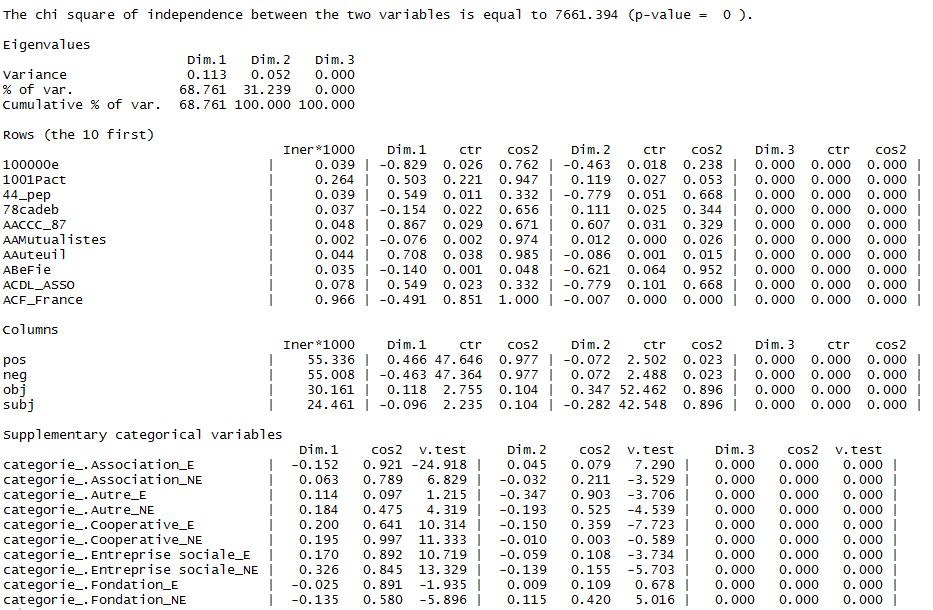
\includegraphics[width=\linewidth]{fig/AFC_summary.JPG}
                }
            \end{figure}

            Par construction, la variance est répartie sur deux axes, l’un correspondant au sentiment, l’autre à l’objectivité. L’axe horizontal (dimension 1) explique 68,76 \% de la variance totale et correspond au sentiment. Les organisations du corpus se distinguent donc principalement selon qu’elles ont recours à un discours majoritairement positif ou majoritairement négatif. L’axe vertical (dimension 2) explique les 32,24 \% de variance restante, qui correspondent à l’opposition entre les tweets objectifs et les tweets subjectifs. Cette distinction est donc nettement moins significative. La Figure \ref{fig:AFCcategories} présente une projection des catégories d’organisations sur ces deux axes. On a ici distingué pour chaque catégorie les organisations environnementales et les organisations non environnementales (ex : Association\_E vs Association\_NE). La qualité de projection est mesurée à l’aide du cosinus carré (cf. figure \ref{fig:syntheseAFC} : colonne cos2), compris entre 0 et 1.

            \begin{figure}
                \caption{Carte factorielle : catégories d'utilisateurs}
                \label{fig:AFCcategories}
                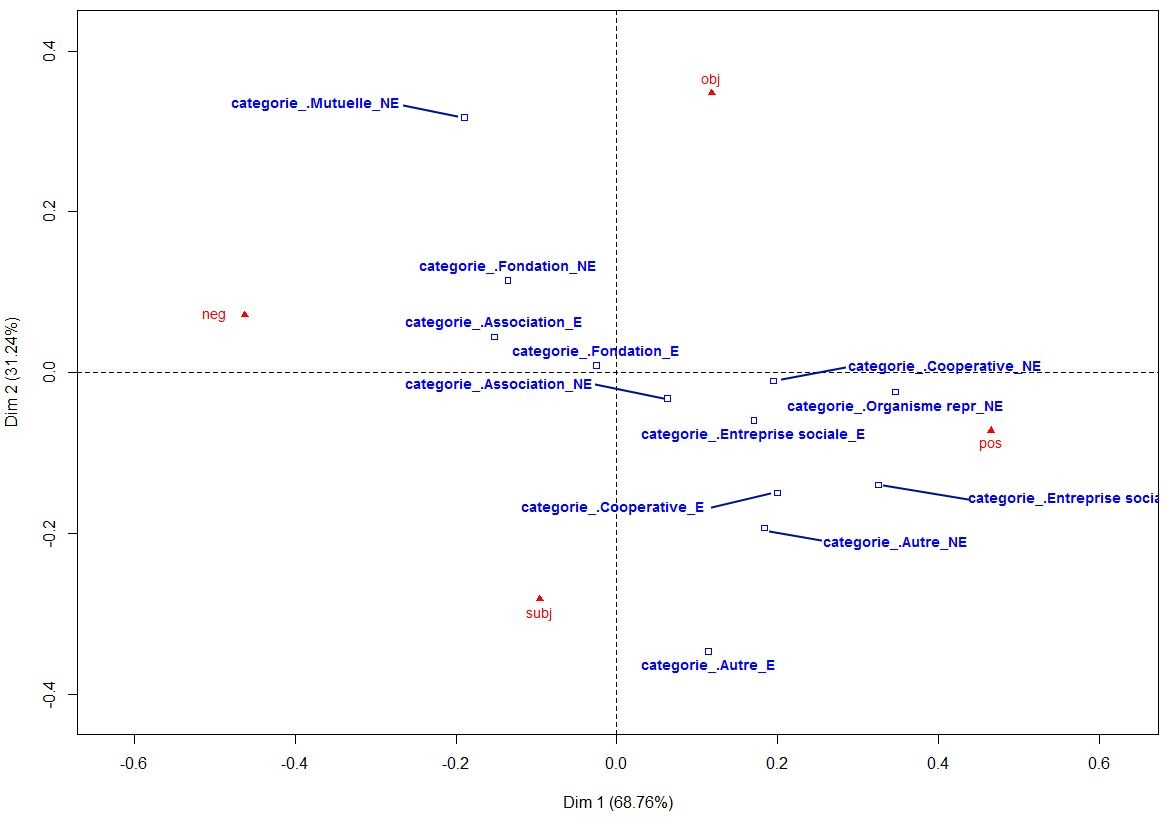
\includegraphics[width=\linewidth]{fig/AFC_categories.JPG}
            \end{figure}

            Les mutuelles se distinguent par un positionnement vers des tweets négatifs mais objectifs. Quelques exemples de tweets nous permettent de comprendre ce discours. Les mutuelles opèrent dans le secteur de la santé et de l’assurance. Par conséquent, elles abordent les thématiques environnementales sur l’angle des risques sanitaires, ceux-ci ayant un impact pour leurs bénéficiaires. L’augmentation des maladies liées à l’environnement pose aussi un risque économique en faisant augmenter les remboursements de frais de santé. Globalement, elles n’adoptent pas une position engagée, mais s’intéressent plutôt aux études publiées sur ces sujets.

            \begin{quotation}
             \citit{La pollution de l’environnement entraîne 1,7 million de décès d’enfants par an https://t.co/gXir1rrLgH} (Mutuelle Apreva, mars 2017)
            \end{quotation}

            A l’opposé, les organismes de représentation adoptent un discours très positif sur la question de l’écologie\footnote{Les valeurs correspondantes n’apparaissent pas sur la Figure 4 qui n’intègre que les 10 premières lignes. La qualité de projection est de 0.995 sur l’axe 1 et 0.005 sur l’axe 2.}. Ce résultat est toutefois à nuancer : cette catégorie représente un petit nombre d’organisations et le nombre de tweets ayant trait à l’environnement est réduit (247 tweets). Les publications concernent des appels à projets, des informations sur des évènements autour des questions environnementales (conférences, ateliers…) ou la valorisation de projets innovants. Ces organisations sont plutôt dans une démarche de promotion de l'\ess et de son action environnementale.

            \begin{quotation}
                \citit{ L'\#ESS s'engage pour la \#transitionénergétique citoyenne ... \#COP21 https://t.co/lGryBHgJnI} (\cress Limousin, décembre 2015) \\
                \citit{Lilo le moteur de recherche qui finance des projets sociaux et environnementaux que vous choisissez ! https://t.co/RZ9U9JsWB1} (\cress Champagne-Ardennes, juin 2016)
            \end{quotation}

            Les associations se distinguent essentiellement sur l’axe horizontal. Elles ont globalement une position centrale, peu discriminante, qui s’explique vraisemblablement par la grande diversité du secteur et donc des positionnements. Les associations environnementales se distinguent toutefois par un discours plus négatif. Elles ont souvent une position engagée, réagissant à l’actualité politique. Elles ont aussi un rôle d’alerte sur les risques environnementaux.

            \begin{quotation}
                \citit{\#Nucléaire: \@RoyalSegolene utilise la \#PPE pour relancer la filière \#MOX. Et les \#déchets, on en fait quoi? Non à l'enfouissement à \#Bure !} (Association amisdelaterre, juillet 2016)
            \end{quotation}

            Concernant les fondations dont la mission est liée à l’environnement, l’AFC ne permet pas d’identifier une stratégie distincte. En revanche, les fondations non environnementales adoptent, de façon similaire mais moins marquée que les mutuelles, un discours plutôt négatif mais objectif. De nombreuses fondations opérant dans le domaine de la santé, ce positionnement peut s’expliquer par les mêmes raisons.

            Un discours majoritairement positif est adopté par les coopératives et les entreprises sociales, qu’elles aient une mission environnementale ou non. Ces organisations se distinguent assez mal sur l’axe vertical, à l’exception des coopératives environnementales associées à un discours sensiblement plus subjectif. Dans le discours des coopératives et des entreprises sociales, l’accent est mis sur les aspects positifs. De nombreux tweets portent sur les avancées en matière environnementale, les progrès effectués, ainsi que les opportunités de développement. De nombreux cas de réussites entrepreneuriales basées sur les questions environnementales sont mis en avant, comme pour démontrer que les alternatives existent et qu’elles se mettent déjà en place. Les tweets jouent aussi un rôle de promotion des actions environnementales menées par les entreprises.

            \begin{quotation}
                \citit{Pr bien commencer 2016, voici 1 reportage d'1 école parisienne qui a déjà pris de bonnes résolutions. https://t.co/yYwNUr6Kcj \#biodéchets} (Entreprise Sociale loveyourwaste, janvier 2016) \\

                \citit{Les producteurs du \@groupedaucy en route vers l'\#Agroecologie \#sustainableagriculture https://t.co/hGqfJZzMaz } (groupedaucy, coopérative novembre 2016)
            \end{quotation}

            L’analyse des axes peut être facilitée par la visualisation des cas les plus significatifs. La figure \ref{fig:AFCentreprises} fait apparaitre les 30 comptes Twitter ayant la plus forte contribution à la construction des axes.

            Dans le cadran supérieur gauche, l’association Airparif se distingue par un discours objectif mais essentiellement négatif. Ce compte Twitter publie régulièrement une information sur le niveau de pollution en Ile de France… souvent élevé, mais qui relève d’une mesure parfaitement objective.  Plus bas, la Fondation du Souffle (\textit{FduSouffle}), qui rassemble des acteurs de la lutte contre les maladies respiratoires se distingue assez logiquement par un discours négatif, la pollution étant une des causes de ces maladies.

            Le cadre inférieur gauche fait apparaitre un groupe d’associations associées à un discours plutôt négatif, dont WWF France, Oxfam France (\textit{oxfam\_fr}), GreenPeace (\textit{greenpeacefr}) et Sortir du Nucléaire France (\textit{sdnfr}). Ces associations ont un rôle d’activisme sur les questions environnementales (à l’exception d’Oxfam qui lutte contre la pauvreté mais s’exprime aussi sur l’écologie). Elles adoptent parfois un rôle de lanceur d’alerte, en signalant les projets allant à l’encontre de la transition écologique et en alertant sur les dangers pour les citoyens. Ces organisations prennent fréquemment des positions politiques en lien avec l’actualité.


            \begin{quotation}
                \citit{Richesse et revenus extrêmes sont inefficaces économiquement et nuisent à l’environnement, selon 1 rapport http://t.co/xrtYothI} (Oxfam France, janvier 2013) \\
                \citit{Environnement: le programme \#Macron est incohérent et ne remet pas en cause le système actuel désastreux \#TelSonne https://t.co/iJgbPWaeCa} (GreenPeace France, avril 2017) \\
                \citit{Important rejet radioactif à centrale \#nucléaire de Golfech (82), déclaré presque 1 semaine + tard : notre réaction https://t.co/S8gUiHBxuE} (Sortir du Nucléaire France, octobre 2016)

            \end{quotation}


            \begin{figure}
                \caption{Carte factorielle : Utilisateurs significatifs}
                \label{fig:AFCentreprises}
                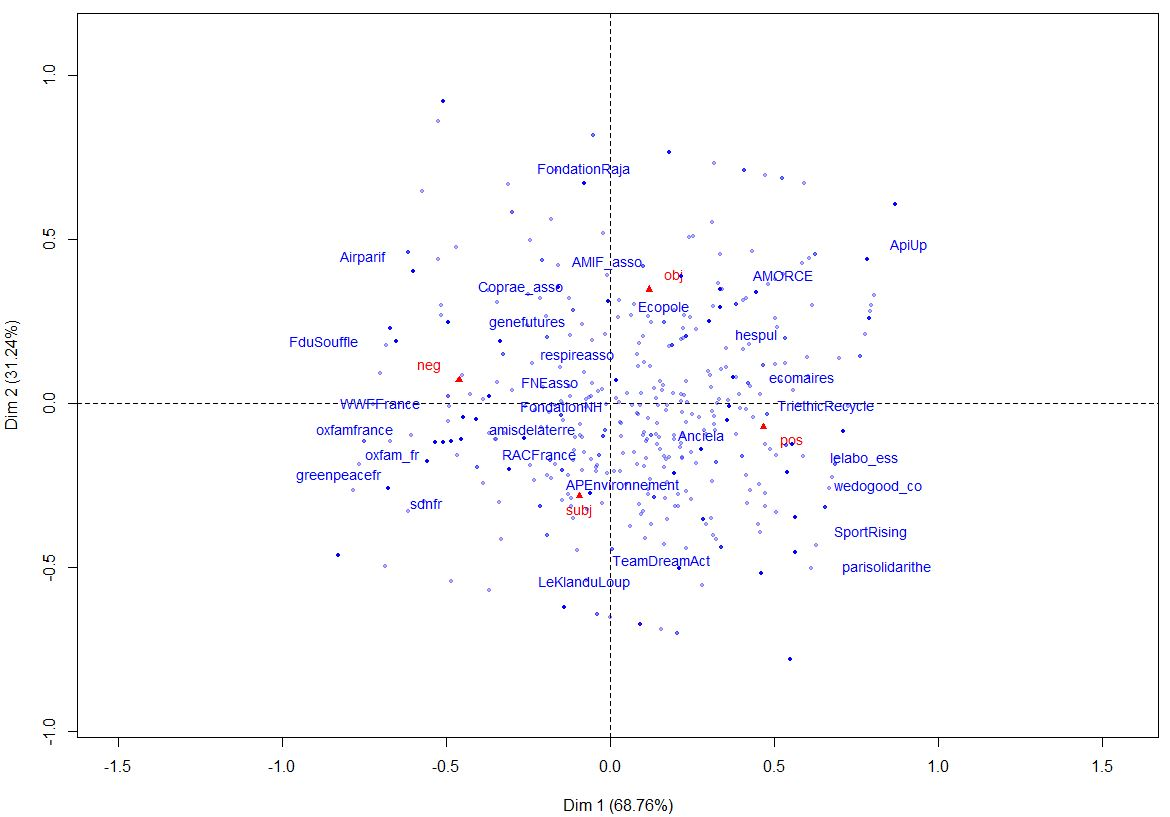
\includegraphics[width=\linewidth]{fig/AFC_entreprises.JPG}
            \end{figure}

            Tout en bas, Le Klan du Loup et TeamDreamAct sont caractéristiques d’un discours majoritairement subjectif, marqué par des interactions importantes avec les utilisateurs et par des prises de positions fortes, usant parfois d’humour, d’ironie ou de sarcasme.


            \begin{quotation}
                \citit{Les trois plaies pour la biodiversité : Chasse, pêche et agriculture \\
                https://t.co/AZ6Yv1iGYT \#biocentrisme \#environnement \#écologie} (Le Klan du Loup, Août 2016) \\
                \citit{"Malgré les intempéries... l'été approche alors ayez la fraîcheur écolo :) https://t.co/YzeQz41UFB https://t.co/vvORveDhqF"} (TeamDreamAct, juin 2016)
            \end{quotation}

            Le cadran inférieur droit correspond aux entreprises adoptant un discours plutôt subjectif mais positif. C’est le cas de parissolidarithe (association membre du \mouves), SportRising (coopérative sous forme de SCOP) ou encore wedogood (entreprise sociale).

            \begin{quotation}
               \citit{Quand le sport se met au service des hommes et de l'environnement! \@LaurentOlmo \@bbarbusse \@DominiqueCrochu  https://t.co/9Rtx40AGDJ} (SportRisin, septembre 2015) \\
                \citit{\@Green\_spector : bravo, toujours au top pour l'efficacité énergétique ! \#greenIT \#transition \#numérique} (wedogood\_co, décembre 2016)

            \end{quotation}



            Enfin, un discours positif et plutôt objectif est adopté par les organisations présentes dans le cadran supérieur droit, comme Amorce, réseau d'information et d'accompagnement en matière d'écologie, ou API'UP, association de récupération et recyclage des déchets.

            \begin{quotation}
               \citit{.\@AMORCE 1 million d'euros d'économie dans les collèges isérois grâce à la lutte contre le \#gapillagealimentaire \#BIO2016} (Amorce, mai 2016) \\
            \end{quotation}

            Dans l'étape suivante, nous proposons une approche plus fine, basée sur la correspondance entre le discours des organisations et des cadres rhétoriques prédéfinis.


        \subsubsection{Étude du cadrage du discours}

            362 hashtags utilisés au moins 15 fois dans le corpus ont été analysés pour être affectés aux huit cadres identifiés par \textcite{nisbet2009communicating}. 111 n’ont pu être affectés à aucun cadre rhétorique. Le tableau \ref{table:21hashtagsnisbet} détaille l’affectation des 251 hashtags qui correspondent à un cadre particulier.\\

            \begin{table}
                \caption{Affectation des hashtags aux registres}
                \label{table:21hashtagsnisbet}
                \footnotesize

                \begin{tabularx}{\linewidth}{|K{0.20\linewidth}|X|}
                \hline

                \textbf{Cadres}	&\textbf{Hashtags}
                \\ \hline

                Conflict and strategy	& enercoop, edf, ouiauxloups, projectrescueocean, antigaspi, confenvi, plantfortheplanet, nddl, legranddebat, colloque, fessenheim, conférence, cashinvestigation, stopcharbon, bure, afp, stoppesticides, macron, lemissionpolitique, congrèsamorce, monsanto, trump, 15minutespourconvaincre, zerodeforestation\\ \hline
                Economic development and competitiveness & 	dd, emploi, innovation, developpementdurable, développementdurable, crowdfunding, startup, économie, développement, entreprise, entreprises, numérique, devdurable, appelaprojets, agroforesterie, emplois, financement, bioéconomie, planification, bâtiment, finance, fiscalité, greentech, travail, economie, agriculteurs, banques, developpement, économique, btp\\ \hline
                Middle way/alternative path	& bio, recyclage, economiecirculaire, durable, zerowaste, transitionenergetique, économiecirculaire, zerodechet, transition, agroécologie, upcycling, transitionénergétique, zérodéchet, photovoltaïque, tri, agroecologie, renouvelable, éolien, circuitscourts, réemploi, circuitcourt, biodéchets, photovoltaique, renouvelables, permaculture, local, transitionecologique, recycler, territoires, biocentrisme, solaire, vélo, biogaz, nuitagroecologie, compostage, alternatives, rénovation, économiesénergie, autoconsommation, diy, palmedurable, mondevivable, collecte, palmedurable, jesuisecoloquand, ecoconception, aménagement, changement, écoquartier, territoire, valorisation, compost, circulaire, smartcity, energiesrenouvelables, vegan, circulareconomy\\ \hline
                Morality and ethics	& rse, responsable, solidaire, solidarité, greenwashing, prévention, ecoresponsable, equitable, chasse, sociale, inégalités, congésolidaire, écoresponsable, solidaires, équitable, fairfinance, commerceequitable, don, engagement, solidarite\\ \hline
                Pandora’s box	& déchets, pollution, dechets, déchet, gaspillage, déforestation, pollutiondelair, obsolescence, deforestation, pollutionair, fukushima, gaspillagealimentaire, cancer, waste, obsolescenceprogrammée, victimes, obsolescenceprogrammee, airpollution, perturbateursendocriniens\\ \hline
                Public accountability and governance &	cop21, ess, energiecitoyenne, cop22, loibiodiv, legislatives2017, socent, scop, accorddeparis, ceta, collectivités, associations, association, citoyen, ecophyto, scic, cop20, ue, loi1901, coop, citoyenne, g7, coopérative, presidentielle2017, loi, tafta, coopératives, servicecivique, citoyenneté, asso\\ \hline
                Scientific and technical uncertainty &	climat, énergie, pesticides, biodiversité, nucléaire, charbon, énergétique, energie, climatechange, huiledepalme, air, eau, biodiversite, énergies, changementclimatique, nucleaire, climatique, climateinitiative, emballages, électricité, ogm, pêcheprofonde, pétrole, gazdeschiste, oceanclimax, nucléaires, papier, climatdatalab, glyphosate, plastique, nanoparticules, gaz, co2, méthanisation, pesticide, epr, réchauffementclimatique, qualitéair, océan, rechauffementclimatique, plastiques, ges, réchauffement, abeilles, néonicotinoïdes, qualiteair, réseauxdechaleur\\ \hline
                Social Progress	& agriculture, santé, sport, alimentation, insertion, consommation, social, habitat, genderday, éducation, mobilité, urbanisme, transport, précarité, sante, logement, education, transports, humanitaire, construction, formation, mobilite, alimentaire, pauvreté\\ \hline


                \end{tabularx}
            \end{table}

            On détermine ainsi, pour chaque utilisateur, le nombre de tweets correspondant à chacun des cadres rhétoriques. Ceci prend la forme d’une table de contingence qui donne lieu à une analyse factorielle des correspondances (AFC). \\

            La variable « catégorie d’organisation » ayant 7 modalités, l’AFC répartit la variance sur 6 dimensions. Les deux premières dimensions expliquent à elles seules 88.8\% de la variance (encadré \ref{encadre:6afcsummary}), ce qui est tout à fait suffisant pour l’analyse. La seule première dimension factorielle correspond à 58.6\% de variance. La figure \ref{figure:7AFC} représente la projection des variables sur les deux premières dimensions. L’interprétation de cette carte factorielle est complétée par les données présentées dans l’encadré \ref{encadre:6afcsummary}, qui détaille la contribution de chaque modalité à la contribution des deux axes (ctr), ainsi que sa qualité de projection (cos2). \\


            \begin{encadre}
                \caption{Synthèse de l’AFC}
                \label{encadre:6afcsummary}
                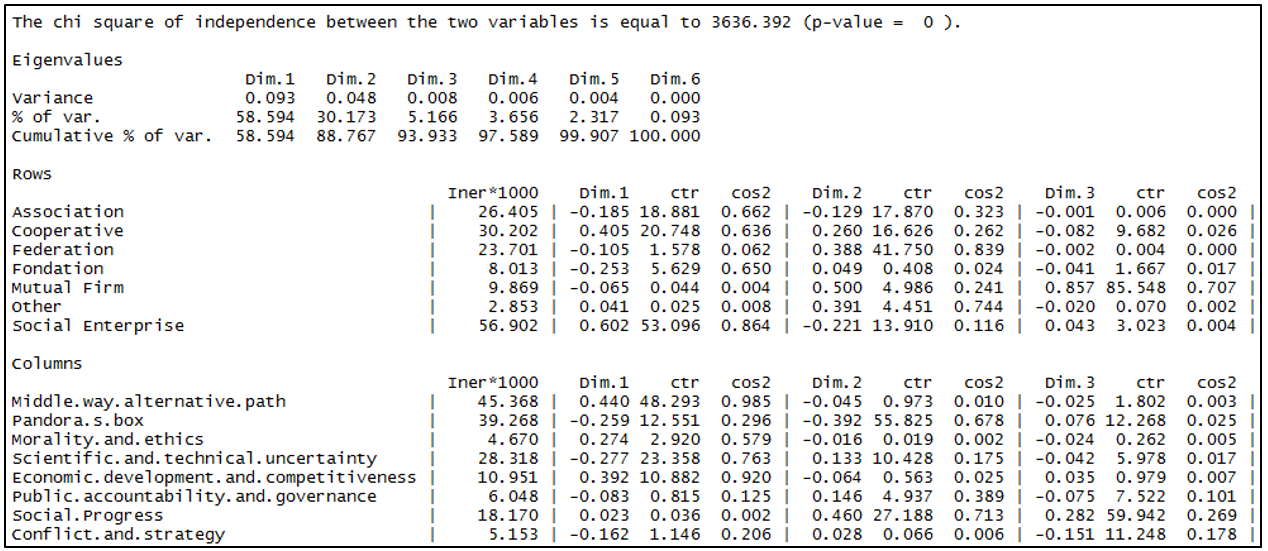
\includegraphics[width = \textwidth]{fig/fig6.png}
            \end{encadre}


            \textbf{La première dimension} est la plus importante et explique 58 \% de la variance. Elle oppose les coopératives et entreprises sociales (coordonnées positives) aux associations et fondations (coordonnées négatives). Les premières mobilisent particulièrement les registres du développement économique / compétitivité et des alternatives / compromis. Les secondes ont davantage recours au registre de l’incertitude scientifique et technologique, et de manière un peu moins nette à celui de la boîte de Pandore et celui des conflits et stratégie. L’axe horizontal oppose ainsi des organisations qui lient le discours environnemental avec une recherche d’opportunités d’innovation et de développement économique, à des organisations qui s’intéressent à l’état scientifique des choses, c’est-à-dire à l’avancement des connaissances relatives à l’écologie. Le secteur non lucratif (associations et fondations) semble aussi plus pessimiste et plus prompt à mettre en avant le danger que fait peser la situation environnementale et à ouvrir un débat critique sur ces questions. \\

            \begin{landscape}
            \begin{figure}
                \caption{Correspondance entre organisations et registres : carte factorielle}
                \label{figure:7AFC}
                \centering
                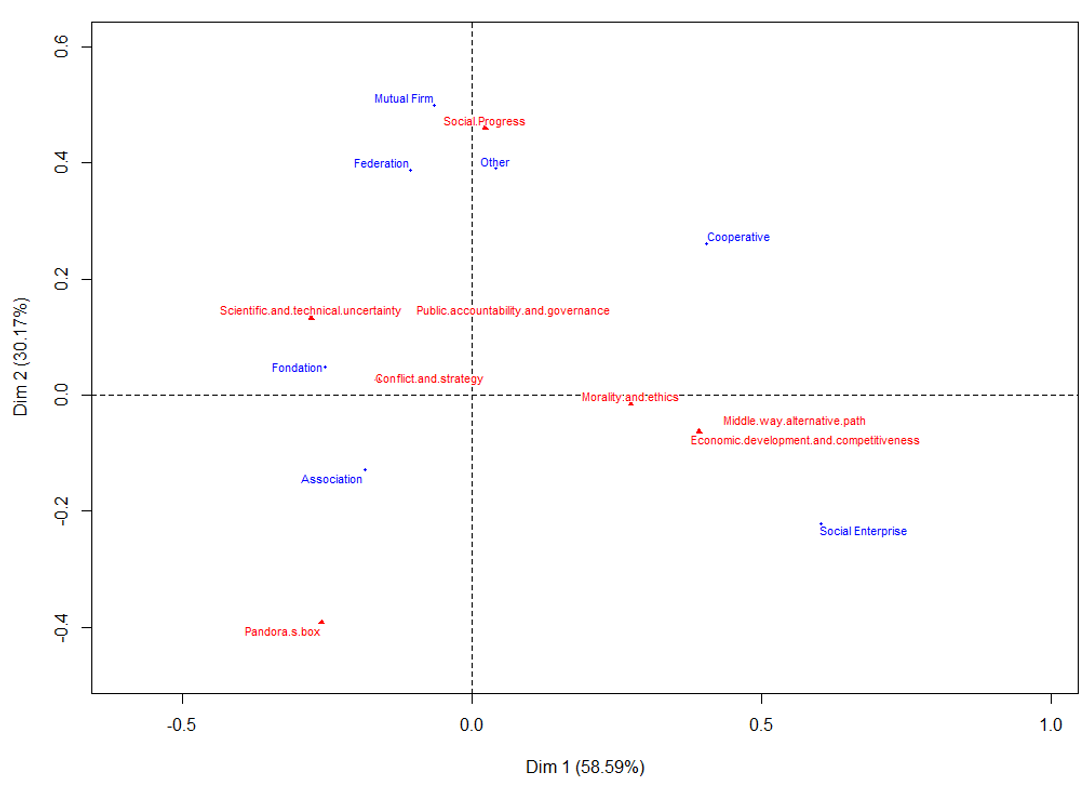
\includegraphics[height = 0.90\textheight]{fig/fig7.png}
            \end{figure}
            \end{landscape}


            \textbf{La seconde dimension factorielle} correspond à 30 \% de la variance totale. Elle met en évidence une correspondance significative entre les mutuelles et fédérations ainsi que la catégorie « autre » (c’est-à-dire les incubateurs et comptes Twitter de marques ou d’évènements) et le cadre du Progrès Social. Le cadre de la Responsabilité publique et de la gouvernance est aussi nettement associé à ces organisations. Il est intéressant d’observer que les coopératives, bien que moins fortement associées à ces cadres, les utilisent davantage que les entreprises sociales et, de façon assez surprenante, que les associations.

            La proximité avec le cadre du Progrès Social s’explique notamment par la mission première des mutuelles qui opère dans le secteur de la santé et de la protection sociale. Elles plébiscitent donc les hashtags relatifs à ce cadre. La même explication peut s’appliquer à la catégorie Fédérations, qui intègre un grand nombre de fédérations mutualistes. Le discours environnemental de ces organisations est donc fortement lié aux questions sociales et sociétales. \\

            Le cadre de la Responsabilité publique et de la gouvernance renvoie à la fois à des questions de politiques publiques et à la gouvernance des entreprises. Or, l’ESS est marquée par des modes de gouvernance particuliers, reposant sur une logique participative et démocratique. Ceci est particulièrement vrai dans les mutuelles qui appartiennent à leurs clients, et dans les coopératives qui peuvent être détenues par différents groupes de parties prenantes. \\

            A l’inverse, associations et entreprises sociales sont ici plus fortement associées avec le cadre de la Boite de Pandore. Ceci ne signifie pas que les associations ne se préoccupent pas de progrès social ou de gouvernance, mais que ces cadres ne sont pas utilisés conjointement au discours environnemental. Comme observé pour la première dimension, les associations utilisent plutôt un cadre « dramatique » pour promouvoir la transition écologique.  \\

            \textbf{La troisième dimension factorielle} n’est pas représentée sur la figure \ref{figure:7AFC}, mais elle présente une meilleure qualité de projection des mutuelles qui confirme la correspondance avec le cadre du Progrès Social (encadré \ref{encadre:6afcsummary}).




    \subsection{Etude de la performance des tweets }

        \subsubsection{Selon le cadrage rhétorique}

            L’AFC montre que les différentes formes organisationnelles de l’ESS ont recours à des cadres rhétoriques différents pour porter le discours environnemental. Ceci conduit à se demander lesquels sont les plus efficaces pour permettre la diffusion des idées véhiculées dans les tweets. Pour mesurer cette performance, deux indicateurs sont utilisés : le nombre de retweets et le nombre de favoris. Pour chaque cadre rhétorique, le tableau \ref{table:22rtmean} indique le nombre moyen de retweets et de mise en favoris des tweets.

            \begin{table}
                \caption{Nombre moyen de retweets et de favoris en fonction du cadre rhétorique}
                \label{table:22rtmean}
                \centering
                \small
                \begin{tabularx}{\textwidth}{|X|R|R|}
                    \hline
                    \head{Cadre rhétorique}&	\head{Nombre de retweets}&	\finalhead{Nombre de favoris} \\ \hline

                    Conflict and strategy&	16.10	&10.88 \\ \hline
                    Scientific and technical uncertainty&	8.83&	5.09\\ \hline
                    Public accountability and governance&	6.70&	4.10\\ \hline
                    Pandora’s box&	4.69&	2.25\\ \hline
                    Morality and ethics	&3.54&	2.26\\ \hline
                    Middle way/alternative path&	3.18&	2.86\\ \hline
                    Social Progress	&2.97&	2.24\\ \hline
                    Economic development and competitiveness&	2.29&	1.95\\ \hline

                \end{tabularx}
            \end{table}


            Le cadre « Conflit et stratégie » semble nettement plus performant que les autres, avec plus du double de retweets par rapport au second registre (Incertitude scientifique et technique). Les cadres « Incertitude scientifique et technique » et « Responsabilité publique et gouvernance » sont également performants. Ils correspondent, pour le premier, aux hashtags renvoyant au niveau actuel de la connaissance sur les questions d’écologie, et pour le second, aux questions de décisions publiques et de responsabilité des gouvernements, des entreprises et des individus.

            Bien que les tweets recourant au cadre de la « Boite de Pandore » soient moins retweetés, ils sont toutefois plus performants que les tweets concernant la morale, les alternatives, le progrès social ou le développement économique.  \\

            Une limite à cette lecture statistique est que ces deux variables font ressortir un certain nombre de valeurs extrêmes, c’est-à-dire des tweets qui ont été massivement partagés ou mis en favoris et qui viennent gonfler la moyenne. Or, il n’est pas pertinent d’éliminer ces outliers, car c’est précisément cet « effet buzz » qui est recherché sur les réseaux sociaux afin de diffuser le plus efficacement un contenu. On cherche au contraire à déterminer dans quel cadre rhétorique s’inscrivent les tweets qui ont bénéficié de cet effet. Pour cela, le tableau \ref{table:23toptweets} présente les 20 tweets ayant été le plus retweetés sur le réseau social. Il s’agit essentiellement de tweets très engagés et critiques, utilisant des mécanismes rhétoriques comme l’ironie ou le sarcasme. Ils s’inscrivent dans une logique d’interpellation en mentionnant ou en s’adressant directement à des responsables politiques. Les tweets peuvent aussi s’adresser à des grandes entreprises, mises en cause pour leur comportement vis-à-vis de l’environnement. L’urgence d’agir est aussi mise en avant dans ces tweets, ainsi que le danger engendré par certaines pratiques, notamment en lien avec l’industrie nucléaire. \\


            \begin{landscape}
                \begin{table}
                \caption{Tweets les plus partagés}
                \label{table:23toptweets}
                    \centering
                    \scriptsize
                    \begin{tabularx}{\linewidth}{|L|K{0.8\linewidth}|R|}
                    \hline
                    \head{Auteur}	&	\head{texte}	&	\finalhead{Nombre de retweets}	\\ \hline

                        FondationNH	&	\#Trump : Sortir de l'Accord de Paris c'est un contre-sens tragique de l'histoire!  \#climat https://t.co/XONkeg3fJH	&	1012	\\ \hline
                        oxfamfrance	&	RT cette photo pour rappeler à @fhollande ses engagements sur le \#climat. \#LikeTaPlanete http://t.co/NMmnXPy5M5	&	1000	\\ \hline
                        greenpeacefr	&	Environnement: le programme \#Macron est incohérent et ne remet pas en cause le système actuel désastreux \#TelSonne https://t.co/iJgbPWaeCa	&	829	\\ \hline
                        FondationNH	&	Donald Trump réalise un acte stupide et criminel qui va à rebours du sens de l’Histoire en sortant de l' \#AccorddeParis  \#Trump \#climat	&	501	\\ \hline
                        WWFFrance	&	Malgré une sortie possible de l’\#AccordDeParis, les villes vont intensifier leur action pour le \#climat aux États-U… https://t.co/3WMhAKmf04	&	495	\\ \hline
                        WWFFrance	&	En cette journée mondiale de l'\#environnement, rendons hommage aux poumons de notre planète : les forêts ! ️… https://t.co/Gbg2vh2oWD	&	491	\\ \hline
                        greenpeacefr	&	Impunité des grands pollueurs, drames écologiques en pagaille...et il faudrait se taire ? \#NosVoixSontEssentielles… https://t.co/lv0jSPeJfp	&	338	\\ \hline
                        greenpeacefr	&	Non, le charbon n’a pas remplacé le \#nucléaire en Allemagne. Mensonge @EmmanuelMacron \#AlterQG \#LEmissionpolitique https://t.co/A9Hq7sZD3D	&	328	\\ \hline
                        greenpeacefr	&	\#Fukushima : la France n’a pas tiré les leçons des accidents \#nucléaires. Le danger plus présent que jamais du côté… https://t.co/croQ1NiRbb	&	286	\\ \hline
                        greenpeacefr	&	Pendant que la France s'enfonce dans sa fuite en avant \#nucléaire, les Suisses lui tournent le dos. https://t.co/KXTtk8uGnM via @libe	&	279	\\ \hline
                        RACFrance	&	\#PLF2017: la France doit respecter ses engagements! Augmentez les recettes de la \#TTF pr le développement \& \#climat… https://t.co/RwBNDSbB89	&	275	\\ \hline
                        greenpeacefr	&	Pas un mot d'@EmmanuelMacron sur l'écologie. Étonnant? Pas tant. \#alterQG \#15minutesPourConvaincre https://t.co/iJgbPWaeCa	&	262	\\ \hline
                        greenpeacefr	&	[BREAKING] Scandale anomalies Creusot: des documents prouvent qu' EDF et AREVA étaient alertées dès 2005 \#nucléaire https://t.co/sbAU6D7H1T	&	242	\\ \hline
                        FondationNH	&	\#LoiBiodiv : Le Sénat préfère les pesticides aux abeilles! https://t.co/gC8wrfjNhp  \#neonicotinoides \#biodiversite https://t.co/x8BPdS0jcq	&	227	\\ \hline
                        amisdelaterre	&	Ils reviennent les \#Pinocchio2015 \#climat \& n'échapperont pas à vos votes! A vous de jouer https://t.co/yZCNHJwUYX \newline https://t.co/JRUGW1fT8U	&	225	\\ \hline
                        FondationNH	&	Contre les faits,contre la science, le Sénat refuse d'interdire pesticides \#néonicotinoïdes \#LoiBiodiv \#biodiversité https://t.co/kBeHDB8rrb	&	200	\\ \hline
                        attac\_fr &	Transition sociale et écologique = 0 \newline Lutte contre l'impunité fiscale = 0 \newline \#2017LeDebat	&	190	\\ \hline
                        greenpeacefr	&	La faillite du \#nucléaire, de moins en moins discrète : \#EDF admet un risque de black-out. https://t.co/tnk5uIdSIu https://t.co/Xs86WaTERF	&	187	\\ \hline
                        FNEasso	&	\#NDDL : qui va payer la destruction de l'environnement et la construction d'infrastructures inutiles ? https://t.co/2YKZbNFcj6	&	183	\\ \hline
                        amisdelaterre	&	.@SocieteGenerale \& @BNPParibas soutiennent \#gazdeschiste aux USA. Elles ne peuvent pas le faire ici!… https://t.co/6e0j2ccF6Y	&	178	\\ \hline
                    \end{tabularx}

                \end{table}
            \end{landscape}



            Une bonne performance d’un tweet, soit une bonne visibilité sur le réseau, semble ainsi résulter d’un propos vivement engagé, voire impertinent, appelant à la controverse et au débat et s’appuyant sur l’actualité. Twitter apparaît donc ici comme un réseau social favorisant la polémique, le débat et la prise de position. Le meilleur moyen de promouvoir la transition écologique sur ce réseau est donc d’adopter une posture engagée, quitte à recourir à l’exagération et à prendre à partie les opposants aux idées défendues. Ce sont donc les stratégies de communication adoptées par les organisations à but non lucratif qui semblent les plus efficaces sur Twitter. La communication des coopératives et entreprises sociales, reposant sur des aspects économiques et sur la présentation d’alternatives innovantes, ou celle des mutuelles, basée sur le progrès social, semblent beaucoup moins performantes.  \\

            Cependant, les tweets les plus partagés sont diffusés par des entreprises de l’ESS très connues du grand public et ayant un grand nombre d’abonnés. Or, il a été démontré que le nombre d’abonnés a une forte influence sur la performance d'un tweet. On peut dès lors se demander si les tweets sont performants en raison des cadres rhétoriques qu’ils utilisent, ou bien parce qu’ils sont publiés par des organisations ayant un grand nombre d’abonnés, qui sont aussi plus susceptibles d’utiliser ces cadres. Les organisations ayant le plus grand nombre de tweets (comme la Fondation Nicolas Hulot, GreenPeace, WWF ou Attac) sont en effet connues pour leur engagement militant et leurs prises de positions politiques en faveur de l’écologie. Pour éliminer l’impact de la popularité de l’émetteur, c’est-à-dire de son nombre d’abonnés, on utilise le niveau d'engagement, qui a été défini de la manière suivante (\ref{twitter:perf}) : \\
            \begin{center}
                $Engagement = \dfrac{Nombre\ de\ retweets + Nombre\ de \ favoris}{Nombre\ d'abonnés} \times 1000$ \\
            \end{center}

            La valeur moyenne de cet indicateur est calculée pour chaque cadre rhétorique. Les résultats sont présentés dans le tableau \ref{table:23perfmean}. Le test de Mann-Whitney est utilisé pour déterminer si ces écarts sont significatifs (tableau \ref{table:24MW})\footnote{Ce test non paramétrique nécessite des échantillons de même taille : aussi, une sélection aléatoire de 800 tweets de chaque cadre est effectuée préalablement au test} . Comme précédemment, on applique la correction de Bonferoni (le niveau de significativité est interprété selon la p-value divisée par 28).

            \begin{table}
                \caption{Performance des tweets en fonction du cadre rhétorique}
                \label{table:23perfmean}
                \centering
                \small
                \begin{tabularx}{\textwidth}{|K{0.5\textwidth}|R|}
                    \hline
                    \head{Cadre rhétorique}&	\finalhead{Engagement} \\ \hline

                    Conflict and strategy&	2.59\\ \hline
                    Middle way/alternative path	&2.55\\ \hline
                    Social Progress&	2.07\\ \hline
                    Morality and ethics&2.02\\ \hline
                    Economic development and competitiveness&	2.02\\ \hline
                    Public accountability and governance&	1.89\\ \hline
                    Scientific and technical uncertainty&	1.55\\ \hline
                    Pandora’s box&	1.43\\ \hline


                \end{tabularx}
            \end{table}


            \begin{table}
                \caption{Comparaison de la performance des cadres - test de Mann-Whitney}
                \label{table:24MW}
                \centering
                \scriptsize
                \begin{tabularx}{\linewidth}{|K{2cm}|K{0.3cm}|L|L|L|L|L|L|L|L|}
                \hline
                &&Middle way,  alt. path &	Pandora’s box &	Morality and ethics &	Sci. and tech. uncertainty	& Economic dev. and comp. &	Public account. and gov. &	Social Progress &	Conflict and strategy\\ \hline

                \multirow{2}{=}{Middle way, alt. path}	&	U	&	338106	&	292044***	&	323043	&	309554**	&	305352***	&	267150***	&	295958***	&	333182	\\
                &		p	&	(0.3212)	&	(0.0000)	&	(0.0081)	&	(0.0001)	&	(0.0000)	&	(0.0000)	&	(0.0000)	&	(0.1573)	\\ \hline
                \multirow{2}{=}{Pandora’s box}	&	U	&	291902***	&	331794	&	324866	&	336008	&	326230	&	324744	&	335613	&	299068***	\\
                &		p	&	(0.0000)	&	(0.1192)	&	(0.0178)	&	(0.2446)	&	(0.0218)	&	(0.0236)	&	(0.1925)	&	(0.0000)	\\ \hline
                \multirow{2}{=}{Morality and ethics}	&	U	&	313373*	&	330962	&	341964	&	339855	&	339681	&	326124	&	331795	&	312443*	\\
                &		p	&	(0.0002)	&	(0.0830)	&	(0.5000)	&	(0.4003)	&	(0.3793)	&	(0.0245)	&	(0.0676)	&	(0.0003)	\\ \hline
                \multirow{2}{=}{Sci. and tech. uncertainty}	&	U	&	305983***	&	336454	&	334854	&	337970	&	322920	&	305533***	&	338640	&	309926*	\\
                &		p	&	(0.0000)	&	(0.2672)	&	(0.1964)	&	(0.3260)	&	(0.0096)	&	(0.0000)	&	(0.3410)	&	(0.0002)	\\ \hline
                \multirow{2}{=}{Economic dev. and comp.}	&	U	&	322675	&	341874	&	337290	&	334633	&	340986	&	310761**	&	333553	&	315211	\\
                &		p	&	(0.0095)	&	(0.4957)	&	(0.2695)	&	(0.1960)	&	(0.4504)	&	(0.0000)	&	(0.1112)	&	(0.0009)	\\ \hline
                \multirow{2}{=}{Public account. / gov.}	&	U	&	263358***	&	320946	&	322155	&	329282	&	309356***	&	330485	&	328110	&	296710***	\\
                &		p	&	(0.0000)	&	(0.0053)	&	(0.0064)	&	(0.0689)	&	(0.0000)	&	(0.0861)	&	(0.0283)	&	(0.0000)	\\ \hline
                \multirow{2}{=}{Social Progress}	&	U	&	306896***	&	336084	&	329490	&	331729	&	335453	&	330092	&	339978	&	299813***	\\
                &		p	&	(0.0000)	&	(0.2205)	&	(0.0373)	&	(0.0959)	&	(0.1739)	&	(0.0562)	&	(0.3609)	&	(0.0000)	\\ \hline
                \multirow{2}{=}{Conflict and strategy}	&	U	&	336426	&	304477***	&	310647**	&	291900***	&	320314	&	285108***	&	299272***	&	336144	\\
                &		p	&	(0.2699)	&	(0.0000)	&	(0.0001)	&	(0.0000)	&	(0.0057)	&	(0.0000)	&	(0.0000)	&	(0.2643)	\\ \hline


                \end{tabularx}
            \end{table}


            L’impact du nombre d’abonnés étant éliminé, le cadre « Conflits et stratégie » apparaît toujours comme le plus performant, mais cette fois-ci au même niveau que le cadre des « Compromis et alternatives ». La faible performance de ce dernier cadre dans la précédente analyse vient donc du fait qu’il est plutôt mobilisé par des organisations ayant peu d’abonnés. A nombre d’abonnés égal, ce cadre est donc efficace pour favoriser la diffusion des tweets. Il en va de même pour les cadres du « Progrès social », de la « Moralité et l’éthique » et du « Développement économique et compétitivité. Toutefois, à l’exception des deux cadres les plus performants, les résultats ne montrent pas de différence significative entre les cadres rhétoriques.



         \subsubsection{Selon le sentiment et l'objectivité}
            De la même manière que l'on a étudié la performance des registres rhétoriques utilisés, on peut comparer les performances selon l'usage de tweets positifs ou négatifs, et objectifs ou subjectifs. Les écarts sont présentés dans le tableau \ref{table:perftweet1}.

            Les résultats des tests de comparaison sont très significatifs (tableau \ref{table:perftweet2}), montrant ainsi que les écarts de performance ne sont pas liés à l'erreur d'échantillonage. Les tweets ayant un caractère négatif sont nettement plus retweetés et plus mis en favoris que les tweets positifs. Cependant, une fois éliminé l'effet du nombre d'abonnés, les tweets positifs obtiennent en réalité un taux d'engagement plus élevé. Ceci semble indiquer que si un discours négatif est plus souvent adopté par des organisations ayant un grand nombre d'abonnés, le recours à un discours positif est préférable pour atteindre son audience. Il en va de même avec les tweets objectifs qui obtiennent un meilleur taux d'engagement, bien que les organisations avec un grand nombre d'abonnés obtiennent un fort impact avec des tweets subjectifs.

            \begin{table}[]
            \caption{Performance des tweets selon le sentiment et l'objectivité}
            \label{table:perftweet1}
                \centering
                \small
                \begin{tabularx}{\linewidth}{|K{0.16\linewidth}|R|R|R|R|R|R|}
                    \hline
                    & \multicolumn{3}{|c|}{\textbf{Sentiment}} & \multicolumn{3}{|c|}{\textbf{Objectivité}} \\ \hline

                    & \head{Positif} & \head{Négatif} & \head{Ecart (\%)} & \head{Objectif} & \head{Subjectif} &  \finalhead{Ecart (\%)} \\ \hline

                    \textbf{Engagement} & 28.34 & 20.75 & 37 \% & 26.31 & 22.81 & 15 \% \\ \hline

                    \textbf{Nombre de retweets} & 5.23 & 10.88 & 108 \% & 6.63 & 9.61 & 45 \% \\ \hline

                    \textbf{Nombre de favoris} & 4.66 & 7.81 & 68 \% & 5.01 & 7.21 & 44 \% \\ \hline
                \end{tabularx}
            \end{table}

            \begin{table}[]
            \caption{Performance des tweets selon le sentiment et l'objectivité - tests statistiques}
            \label{table:perftweet2}
                \centering
                \small
                \begin{tabularx}{\linewidth}{
                    |K{0.14\linewidth}
                    |K{0.10\linewidth}
                    |L
                    |L
                    |L
                |}
                    \hline
                    & \head{Test} & \head{Engagement} & \head{Nombre de retweets} & \finalhead{Nombre de favoris} \\ \hline
                    \multirow{4}{*}{Objectivité}
                        & \multirow{2}{*}{Test T}
                            & $T = 8.4829$*** & $T = -13.1571$*** & $T = -10.7853$*** \\
                            & & $p = .000$ & $p = .000$ & $p = .000$ \\ \cline{2-5}
                        & \multirow{2}{*}{Wilcoxon}
                            & $W = 13284236$*** & $W = 7004314$*** & $W = 4775770$*** \\
                            & & $p = .000$ & $p = .000$ & $p = .000$ \\ \hline

                    \multirow{4}{*}{Sentiment}
                        & \multirow{2}{*}{Test T}
                            & $T = 15.8020$*** & $ T = -27.3647$*** & $T = -17.7536$*** \\
                            & & $p = .000$ & $p = .000$ & $p = .000$ \\ \cline{2-5}
                        & \multirow{2}{*}{Wilcoxon}
                            & $W = 13593125$*** & $W = 5722547$*** & $W = 4925017$*** \\
                            & & $p = .000$ & $p = .000$ & $p = .000$ \\ \hline

                \end{tabularx}
            \end{table}




            % \todo[inline]{Pourquoi à la fois un test t et wilcoxon ? Vérifier normalité}
